% Official IEEE Access LaTeX template downloaded 2026-09-05 from
% https://ieeeaccess.ieee.org/authors/preparing-your-article/
% Template archive: ACCESS_latex_template_20260513-1-1.zip
\documentclass{ieeeaccess}
\usepackage{cite}
\usepackage{amsmath,amssymb,amsfonts}
\usepackage{graphicx,textcomp,bm}
\usepackage{booktabs,tabularx,array,multirow}
\usepackage{enumitem,algorithm,algpseudocode}

\makeatletter
\AtBeginDocument{\DeclareMathVersion{bold}
\SetSymbolFont{operators}{bold}{T1}{times}{b}{n}
\SetSymbolFont{NewLetters}{bold}{T1}{times}{b}{it}
\SetMathAlphabet{\mathrm}{bold}{T1}{times}{b}{n}
\SetMathAlphabet{\mathit}{bold}{T1}{times}{b}{it}
\SetMathAlphabet{\mathbf}{bold}{T1}{times}{b}{n}
\SetMathAlphabet{\mathtt}{bold}{OT1}{pcr}{b}{n}
\SetSymbolFont{symbols}{bold}{OMS}{cmsy}{b}{n}
\renewcommand\boldmath{\@nomath\boldmath\mathversion{bold}}}
\makeatother

\newcommand{\SG}{SwitchGLOBE}
\newcommand{\FSG}{Fused Exact SwitchGLOBE}
\newcommand{\FastSG}{FastSwitchGLOBE}
\newcommand{\drop}{\mathrm{DROP}}
\newcommand{\pdr}{\mathrm{PDR}}
\newcommand{\E}{\mathbb{E}}
\newcommand{\R}{\mathbb{R}}
\newcolumntype{Y}{>{\centering\arraybackslash}X}

\begin{document}
\vol{14}
\year{2026}
\history{Date of publication xxxx 00, 0000, date of current version xxxx 00, 0000.}
\doi{10.1109/ACCESS.2026.0000000}

\title{Fused Exact SwitchGLOBE: Exact-Semantics Global-to-Local Policy Distillation With Risk-Switched Predictive Recovery for Decentralized UAV Routing}
\author{\uppercase{Anonymous Author(s)}\authorrefmark{1}}
\address[1]{Affiliation withheld for double-blind draft preparation}
\tfootnote{Funding information will be completed by the authors before submission.}
\markboth{Anonymous Author(s): Fused Exact SwitchGLOBE}{Anonymous Author(s): Fused Exact SwitchGLOBE}
\corresp{Corresponding author: to be completed before submission.}

\begin{abstract}
Flying ad hoc networks require reliable packet-forwarding decisions under rapid topology changes and constrained onboard computation. Global graph policies can learn strong routing preferences, but their information requirements conflict with decentralized forwarding, whereas compact approximations can reduce inference time while degrading delivery. This article presents Fused Exact SwitchGLOBE, a deployment-oriented framework with privileged global training, strict-local execution, risk-switched predictive recovery, and exact-semantics execution fusion. A proximal-policy-optimization graph teacher is used only during training, and its masked preferences are distilled into one-hop normal and predictive student branches. A calibrated local switch uses link margin, estimated lifetime, and onward-connectivity evidence. The fused implementation evaluates each branch once and reuses its logits for the action and diagnostics, removing a legacy repeated-forward path without changing the policy definition. A common-simulator evaluation covers eight methods, five training seeds, 14 held-out or stress scenarios, and 200 episodes per seed--scenario pair. SwitchGLOBE Exact obtains a connected-pair packet delivery ratio of 0.9053 and a deadline-delivery ratio of 0.8376. Against the strongest adapted baseline, the paired gains are 1.84 and 2.23 percentage points, respectively. On an NVIDIA A100-SXM4-40GB, fusion reduces batch-one CUDA p95 decision latency from 10.004 to 5.836 ms. The session's host CPU reaches 2.208 ms. A compact variant reaches 2.005 ms on CUDA but fails the predefined reliability gate. The results show that exact implementation optimization can improve latency without surrendering routing evidence, while approximate acceleration requires joint latency and reliability validation.
\end{abstract}

\begin{keywords}
Decentralized systems, flying ad hoc networks, graph neural networks, inference latency, policy distillation, reinforcement learning, UAV routing.
\end{keywords}

\titlepgskip=-21pt
\maketitle

\section{Introduction}

\PARstart{U}{nmanned} aerial vehicles can form infrastructure-free multihop networks for disaster response, sensing, inspection, and temporary coverage. The routing graph in such a flying ad hoc network (FANET) evolves quickly because relative motion changes both connectivity and link quality. A next hop that offers immediate geographic progress may disappear before transmission or may lead to a relay with no stable onward neighbor. Reliable routing therefore needs enough structural and temporal context to anticipate failure, yet an onboard relay cannot assume continuous access to a global graph, a centralized controller, or unlimited compute.

Reinforcement learning (RL) has been applied to joint trajectory and routing control, age-of-information optimization, trusted routing, topology-aware recovery, graph-based forwarding, and high-speed FANETs \cite{alam2024joint,wu2026aoi,jia2025trusted,cui2022tarraq,zhang2025gat,shou2026adaptive}. These studies demonstrate the value of learned adaptation but leave two related deployment questions. First, can global training information be converted into a policy that uses only the observation available at the forwarding relay? Second, if two local experts are needed to cover ordinary and imminent-link-failure conditions, how should their runtime be engineered and measured without confusing network end-to-end delay with neural decision time?

This work addresses both questions. The proposed method, \SG{}, is learned through a sequence of global-teacher, local-distillation, geographic-prior, predictive-feature, and risk-calibration stages. Its deployed policy contains a normal geographic-residual branch and a predictive-prior branch. The normal branch retains efficient routing in common states; the predictive branch recovers states in which the nominal link is locally unsafe. A calibrated switch uses only local features and the masked branch preferences. No global graph or teacher messages are required during execution.

The systems contribution is \emph{Fused Exact} execution. The original instrumented adapter obtained an action and later recomputed both branches for diagnostics. That implementation performed four branch forwards per routing decision even though the mathematical policy required only one forward of each branch. The fused implementation exposes a single \texttt{decide} operation: it evaluates both branches once, applies the original switch and mask, and returns action metadata from those same logits. Fused Exact is therefore not a smaller approximate model and not an early-exit policy. It is the canonical exact \SG{} model with redundant execution removed.

The study is guided by four research questions:
\begin{enumerate}[leftmargin=*]
\item Does strict-local global-to-local distillation with risk-switched recovery improve delivery reliability over conventional, value-based, and graph-RL references in a common simulator?
\item Which component of the proposed method accounts for the observed improvement, and where does the method fail?
\item How much latency is removed by exact-semantics fusion, and why can a large GPU be slower than its host CPU for batch-one routing?
\item Can a faster distilled or conditionally evaluated policy replace Exact without violating a predeclared delivery-quality gate?
\end{enumerate}

The principal contributions are as follows.
\begin{enumerate}[leftmargin=*]
\item We formulate a strict deployment contract that allows privileged graph information for offline learning but restricts online forwarding to relay-local and one-hop information.
\item We combine a geographic-residual normal policy with a predictive local policy through an interpretable risk switch based on margin, link lifetime, and onward lifetime.
\item We introduce an exact-semantics fusion path that eliminates repeated diagnostic forwards and preserves the branch logits, mask, switch rule, and selected action.
\item We evaluate eight methods over five seeds, 14 scenarios, and 200 episodes per seed--scenario cell, using seed-paired scenario-macro inference and explicit definitions for reliability, conditional delay, an energy proxy, and policy-input footprint.
\item We benchmark CPU and A100 CUDA batch-one execution in the same session and profile device-to-host scalar synchronization. We also report negative results: calibrated early exit is behaviorally accurate on the evaluated trajectories but slower, whereas \FastSG{} is faster but fails the reliability gate.
\end{enumerate}

Figure~\ref{fig:architecture} summarizes the separation between privileged training and decentralized execution.

\begin{figure*}[t]
\centering
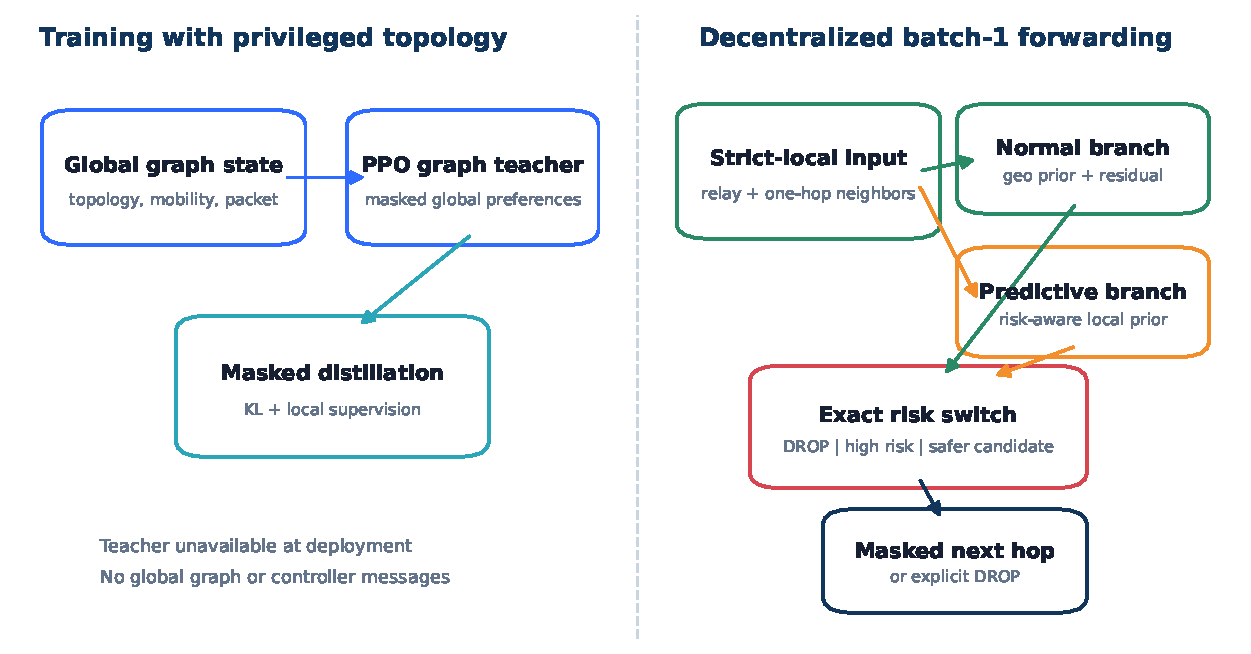
\includegraphics[width=\textwidth]{figures/figure_01_architecture.pdf}
\caption{Overview of \FSG{}. The global graph teacher is confined to training. Both deployed branches use strict-local observations; the exact risk switch returns a masked neighbor or an explicit drop action.}
\label{fig:architecture}
\end{figure*}

\section{Related Work and Research Gap}

\subsection{Learning-Based UAV and FANET Routing}

Topology-aware Q-learning, Q-learning with rate control, and improved multihop Q-learning provide lightweight value-based adaptation \cite{cui2022tarraq,tho2025qlr,sharvari2025improved}. Predictive-Q explicitly couples mobility and interference with dual-path preparation \cite{dong2026predictive}; its reported lightweight decision path motivates our predictive recovery design, but a destination-indexed table and a learned dual-branch policy have different state scaling and runtime behavior. Recent deep RL methods use recurrent DQN, graph attention, multi-agent actors, and broader joint optimization \cite{shou2026adaptive,zhang2025gat,ke2024distributed,wang2025graph}. The UAV literature therefore establishes that topology and motion prediction matter, but it does not by itself guarantee decentralized observability or low batch-one inference latency.

Some methods optimize substantially broader actions. Joint trajectory, frequency allocation, routing, scheduling, power, or buffering can improve a system objective \cite{alam2024joint,wu2026aoi,wang2025graph,zheng2026dual}. These settings are complementary, not numerically interchangeable, with per-hop next-hop selection. Similarly, resilient cluster maintenance and routing in harsh environments provides strong venue-level evidence that graph RL is relevant to UAV resilience \cite{sun2026harsh}, but its cluster-level maintenance objective differs from our exact local forwarding contract.

\subsection{Deployment and Latency Reporting}

Only a minority of the 45 records in the project literature database reports a scoped routing-decision runtime. Many report network end-to-end delay, which includes queueing, medium access, retransmission, propagation, and multihop forwarding. RLFR includes a Raspberry Pi 4B testbed and local forwarding design \cite{li2024rlfr}; RoutePPO reports an eBPF/P4 forwarding-plane update path \cite{curmen2026routeppo}; an ultra-high-speed recurrent method reports online decision time \cite{shou2026adaptive}; and Predictive-Q reports both per-packet and per-slot computational quantities \cite{dong2026predictive}. Hardware, batch size, synchronization, and timed scope are not uniform. Consequently, those values are contextual references rather than fair direct baselines for the present PyTorch policy.

Figure~\ref{fig:litcoverage} visualizes the metric imbalance. The database count is a project audit, not a systematic-review meta-analysis: tags are inherited from the curated records, and the decision-latency count was manually restricted to explicitly scoped compute or forwarding decisions.

\begin{figure*}[t]
\centering

\includegraphics[width=0.88\textwidth]{figures/figure_05_literature_coverage.pdf}
\caption{Metric coverage in the 45-paper project corpus. Generic network delay is common, while directly scoped decision latency is uncommon.}
\label{fig:litcoverage}
\end{figure*}

\subsection{Positioning and Novelty Boundary}

Table~\ref{tab:novelty} states the novelty boundary conservatively. The work does not claim the first use of RL, graph encoders, policy distillation, prediction, or conditional computation in isolation. Its contribution is their deployment-constrained composition and the exact-versus-approximate validation discipline.

\begin{table*}[t]
\caption{Claim--gap matrix used to delimit the contribution.}
\label{tab:novelty}
\centering\small
\begin{tabularx}{\textwidth}{p{0.19\textwidth}p{0.28\textwidth}p{0.25\textwidth}X}
\toprule
Literature capability & Remaining gap & Proposed element & Evidence in this paper \\
\midrule
Graph or multi-agent RL & Global or exchanged state may be required online & Privileged teacher, strict-local student & Observation contract and ablation \\
Predictive or dual-path routing & Prediction can add cost or override a sound nominal action & Calibrated risk-switched predictive recovery & Scenario heatmap and component effects \\
Compact learned routing & Faster approximation can alter route outcomes & Predeclared reliability gate & Exact--Fast paired five-seed test \\
GPU inference & Large accelerators are often assumed to be faster & Synchronized batch-one CPU/CUDA scope & Same-session A100 benchmark \\
Instrumented policy adapters & Diagnostic work can duplicate inference invisibly & Exact-semantics tensor reuse & Legacy--fused equivalence and latency \\
\bottomrule
\end{tabularx}
\end{table*}

\section{System Model and Problem Formulation}

\subsection{Dynamic FANET and Local Action Space}

At decision step $t$, the network is a dynamic graph $\mathcal{G}_t=(\mathcal{V},\mathcal{E}_t)$. A directed edge $(u,v)\in\mathcal{E}_t$ indicates that relay $u$ can currently attempt a transmission to $v$. For a packet with destination $d$, the action space at relay $u$ is
\begin{equation}
\mathcal{A}_u(t)=\mathcal{N}_u(t)\cup\{\drop\},
\end{equation}
where $\mathcal{N}_u(t)$ is the set of reachable one-hop neighbors. Padding permits a fixed maximum number of candidates, and a Boolean mask $M_u(t)$ excludes padding, disconnected candidates, and prohibited actions. The explicit $\drop$ action prevents an invalid padded index from being interpreted as a relay.

The teacher observes a privileged state $s_t$ that may contain the full graph, positions or motion states, link features, the current relay, destination, and packet context. The deployed student receives
\begin{equation}
o_u(t)=\big(x_u, x_d, x_p, \{x_v,x_{uv},f_v,r_v\}_{v\in\mathcal{N}_u(t)},M_u\big),
\end{equation}
where $x_u$, $x_d$, and $x_p$ are relay, destination, and packet features; $x_v$ and $x_{uv}$ are neighbor and link features; $f_v$ denotes bounded forwardability features; and $r_v=[m_v,\ell_v,q_v,o_v]$ contains normalized link margin, current-link lifetime, queue headroom, and best-onward-link lifetime. The deployment contract excludes the full adjacency matrix, remote hidden states, and teacher queries.

\subsection{Objective and Constraints}

Let $Y_e\in\{0,1\}$ denote delivery in episode $e$, $C_e\in\{0,1\}$ indicate that the source--destination pair was initially connected, and $D_e$ denote delivery before a deadline. We seek a local policy that maximizes reliability and deadline delivery while controlling delay and execution cost:
\begin{align}
\max_{\pi} \quad
& \E[\pdr_C(\pi)] + \lambda_D\E[\mathrm{DDR}(\pi)] \notag\\
& {}-\lambda_L\E[L_{95}(\pi)]-\lambda_E\E[E_{\mathrm{proxy}}(\pi)],\\
\text{s.t.}\quad
& a_t\in\mathcal{A}_u(t),\quad \pi(a_t|o_u(t)), \notag\\
& T_{\mathrm{dec},95}\leq B_T.
\end{align}
This multi-objective expression describes the design goal; training uses staged PPO and distillation losses rather than a single scalar solution of the constrained program. Approximate speed variants are judged by a separate acceptance rule. If $\Delta_C$ and $\Delta_D$ are seed-paired changes relative to Exact, a candidate is eligible only if
\begin{equation}
\mathrm{LCB}_{0.95}(\Delta_C)\geq-0.005,\qquad
\mathrm{LCB}_{0.95}(\Delta_D)\geq-0.005,
\label{eq:gate}
\end{equation}
and delay and energy show no material directional degradation.

\section{Proposed Method}

\subsection{Privileged Global PPO Teacher}

The graph-aware teacher is trained offline using proximal policy optimization (PPO) \cite{schulman2017ppo}. Given advantage estimate $\hat A_t$, probability ratio $\rho_t(\theta)$, and clip parameter $\epsilon$, its actor loss is
\begin{equation}
\mathcal{L}_{\mathrm{PPO}}(\theta)=-\E_t\!\left[\min\left(\rho_t\hat A_t,\operatorname{clip}(\rho_t,1-\epsilon,1+\epsilon)\hat A_t\right)\right].
\end{equation}
The same local validity mask used by the student is applied to the teacher's candidate logits before probabilities are produced. The teacher is a source of preferences, not an optimal-route oracle and not a deployment dependency.

\subsection{Masked Global-to-Local Distillation}

For temperature $\tau$, the teacher and student masked distributions are
\begin{equation}
\begin{aligned}
p_T^\tau(a)&=\operatorname{softmax}\!\left(\frac{z_T(a)+\log M(a)}{\tau}\right),\\
p_S^\tau(a)&=\operatorname{softmax}\!\left(\frac{z_S(a)+\log M(a)}{\tau}\right).
\end{aligned}
\end{equation}
The principal distillation term is \cite{hinton2015distilling}
\begin{equation}
\mathcal{L}_{\mathrm{KD}}=\tau^2D_{\mathrm{KL}}(p_T^\tau\Vert p_S^\tau).
\end{equation}
Auxiliary masked cross-entropy terms may supervise teacher action, shortest-path action, and risk-aware local action. Dataset partitions are made by scenario and episode seed, rather than by individual hops, so that transitions from one trajectory do not leak across partitions.

\subsection{Normal Geographic-Residual Branch}

For candidate $v$, let $\Delta d_v=d(u,d)-d(v,d)$ be geographic progress. A shared local encoder $h_\theta(o_u,v)$ and pooled neighbor context $\bar h$ generate a residual score $r_\theta(o_u,v)$. With a learnable positive prior scale $\alpha$ and forwardability feature $f_v$, the normal logit is
\begin{equation}
z^N_v=\alpha\Delta d_v+w_f^\top f_v+r_\theta(o_u,v).
\end{equation}
The residual corrects greedy behavior while the prior provides a stable inductive bias. The branch also emits an explicit drop logit, and the structural mask is applied after all scores are assembled.

\subsection{Predictive Local Branch}

The predictive branch uses the risk vector $r_v=[m_v,\ell_v,q_v,o_v]$. Its implementation is calibrated as a predictive-prior-only branch: the learned residual contribution is set to zero after checkpoint loading, preventing a learned residual from overriding a strong imminent-link-break signal. For calibrated gates $\gamma_m=0.04$, $\gamma_\ell=0.20$, and $\gamma_o=0.20$, candidate danger is
\begin{equation}
D(v)=[\gamma_m-m_v]_+ + [\gamma_\ell-\ell_v]_+ + [\gamma_o-o_v]_+.
\label{eq:danger}
\end{equation}
Queue headroom is available to the predictive prior but is intentionally not part of the switch danger in the verified implementation. This distinction matters for source-to-code consistency.

\subsection{Exact Risk Switch}

Let $a_N=\arg\max_a z^N_a$ and $a_P=\arg\max_a z^P_a$ after masking. Define the safety gain
\begin{equation}
G(a_P,a_N)=(m_{a_P}+\ell_{a_P}+o_{a_P})-(m_{a_N}+\ell_{a_N}+o_{a_N}).
\end{equation}
For switch threshold $\eta=0.05$, the predictive branch is selected when at least one neighbor exists and
\begin{equation}
S=\mathbf{1}\!\left[
\begin{aligned}
&a_N=\drop\;\lor\;D(a_N)>\eta\\
&{}\lor\big(a_P\neq a_N\land G(a_P,a_N)>0.10\\
&\hspace{3.9em}{}\land D(a_P)<D(a_N)\big)
\end{aligned}
\right].
\label{eq:switch}
\end{equation}
The final logits are $z=(1-S)z^N+Sz^P$, followed by the unchanged action mask and softmax. Thus the switch protects the ordinary branch from unnecessary replacement but allows predictive recovery for a drop, a risky nominal link, or a demonstrably safer alternative.

\subsection{Fused Exact Execution}

Figure~\ref{fig:fusion} distinguishes the policy from its runtime wrapper. The legacy instrumented path first obtained the action and then invoked diagnostics that recomputed both branch policies. Fused Exact returns a structured decision containing output logits, switch state, normal and predictive actions, normal probabilities, and diagnostics. Every diagnostic is computed from already available tensors.

\begin{figure*}[t]
\centering

\includegraphics[width=\textwidth]{figures/figure_02_fusion.pdf}
\caption{Legacy repeated execution versus Fused Exact. Fusion removes duplicate branch evaluations; it does not prune a branch or approximate its logits.}
\label{fig:fusion}
\end{figure*}

\textbf{Exactness proposition.} Assume deterministic evaluation mode, identical observations and parameters, and a legacy wrapper whose repeated diagnostic calls do not mutate policy state. Then Fused Exact returns the same masked logits, action, switch indicator, and deterministic diagnostics as the mathematical two-branch \SG{} policy.

\textit{Justification.} The normal and predictive modules are pure deterministic mappings in evaluation mode. Re-evaluating either mapping produces the same logits. Replacing the second evaluations with references to the first logits therefore leaves Equations~\eqref{eq:danger}--\eqref{eq:switch}, the final mask, and all diagnostics unchanged. The implementation is additionally protected by regression tests that count branch forwards and compare replayed outcomes. This is an implementation equivalence argument, not a claim of equivalence under stochastic training mode or stateful layers.

Algorithm~\ref{alg:fused} gives the deployed decision path.

\begin{algorithm*}[t]
\caption{Fused Exact SwitchGLOBE decision}\label{alg:fused}
\begin{algorithmic}[1]
\Require local observation $o$, action mask $M$, normal policy $\pi_N$, predictive policy $\pi_P$
\State $z^N,p^N\gets\pi_N(o)$ \Comment{one normal forward}
\State $z^P,p^P\gets\pi_P(o)$ \Comment{one predictive forward}
\State $a_N\gets\arg\max \operatorname{mask}(z^N,M)$; $a_P\gets\arg\max \operatorname{mask}(z^P,M)$
\State compute $D(a_N)$, $D(a_P)$, and $G(a_P,a_N)$ from local risk features
\State $S\gets$ Equation~\eqref{eq:switch}
\State $z\gets\operatorname{where}(S,z^P,z^N)$
\State $\tilde z\gets\operatorname{mask}(z,M)$; $p\gets\operatorname{softmax}(\tilde z)$
\State derive diagnostics from $z^N,z^P,a_N,a_P,S$ without another forward
\State \Return $\arg\max\tilde z$, $p$, $S$, diagnostics
\end{algorithmic}
\end{algorithm*}

\subsection{Runtime Model and Candidate Optimizations}

Decision time is decomposed as
\begin{equation}
\begin{aligned}
T_{\mathrm{dec}}={}&T_{\mathrm{pre}}+T_N+T_P+T_{\mathrm{gate}}+T_{\mathrm{mask}}\\
&{}+T_{\mathrm{extract}}+T_{\mathrm{sync}}+T_{\mathrm{runtime}}.
\end{aligned}
\end{equation}
Component timers diagnose bottlenecks but are not added to reconstruct end-to-end time because their instrumentation and synchronization boundaries differ. The primary statistic times the complete observation-to-action call.

Three alternatives were tested. Buffered Exact reuses input-tensor storage. Calibrated Early Exit evaluates only the normal branch when its chosen candidate is not drop, a live candidate exists, and $D(a_N)=0$. Its expected time is
\begin{equation}
\E[T_{EE}]=T_N+(1-p_{\mathrm{skip}})T_P+T_g,
\end{equation}
so it helps only if $T_g<p_{\mathrm{skip}}T_P$. \FastSG{} distills Exact into a compact single-pass network. It changes the policy family and must therefore pass Equation~\eqref{eq:gate}; it cannot inherit Exact's behavioral evidence merely because it is trained from Exact.

\section{Experimental Methodology}

\subsection{Common-Simulator Routing Evaluation}

The full comparison uses eight policies: AODV, OLSR, Greedy Geographic, adapted Evo-QGeo, adapted RDQN-HERP, GAT-GRU-DDQN, \FastSG{}, and \SG{} Exact. ``Adapted'' means that the published organizing idea was implemented inside the common simulator; the values are not copied from the original papers and should not be read as a reproduction of their reported testbeds. All methods receive the simulator information permitted by their contracts and use the same episode and scenario schedule.

Five training seeds (42, 77, 123, 314, and 2718), 14 held-out or stress scenarios, and 200 episodes per seed--scenario cell produce 14,000 episodes per method and 112,000 episode rows in the combined archive. Scenarios cover nominal held-out mobility, stochastic link loss, high or extreme mobility, sparse connectivity, node-count shifts, structural geographic holes, predictive breaks, and predictive breaks with loss. Figure~\ref{fig:protocol} summarizes the design.

\begin{figure*}[t]
\centering

\includegraphics[width=\textwidth]{figures/figure_04_protocol.pdf}
\caption{Evaluation protocol. The seed, not the individual packet decision, is the primary inferential unit.}
\label{fig:protocol}
\end{figure*}

\subsection{Metrics and Scope}

For episode set $\mathcal E$, connected-pair PDR is
\begin{equation}
\pdr_C=\frac{\sum_{e\in\mathcal E}Y_e C_e}{\sum_{e\in\mathcal E}C_e},
\end{equation}
and overall PDR is $|\mathcal E|^{-1}\sum_e Y_e$. Deadline delivery ratio is $|\mathcal E|^{-1}\sum_e D_e$. The p95 successful delay is the 0.95 quantile of forwarding steps among delivered packets only. A missing-delivery cell is reported as N/A, never as zero; otherwise a policy that drops every packet could appear to have zero delay. Network end-to-end delay in steps and local decision latency in milliseconds are deliberately reported as different metrics.

Energy per delivered packet is a simulator proxy that aggregates modeled transmission cost and a failure penalty under the synthesis aggregation. It is not a physical Joule measurement. Mean policy-input bytes is the in-memory tensor footprint consumed by the policy and is not wireless control-plane overhead. These qualifications are repeated in the tables because removing the scope would create invalid cross-paper claims.

\subsection{Statistical Analysis}

Episode outcomes are first aggregated within each seed and scenario, then averaged across the 14 scenarios. The primary reported mean is therefore a five-seed scenario-macro estimate. For method $A$ and reference $B$, a directional paired difference is $d_s=x_{A,s}-x_{B,s}$ for higher-is-better metrics and $d_s=x_{B,s}-x_{A,s}$ for lower-is-better metrics. A two-sided 95\% Student-$t$ interval is formed across the five paired seed differences. Deterministic bootstrap intervals and exact sign-flip checks are retained in the latency analysis. With five pairs, the smallest attainable two-sided exact sign-flip $p$-value is $2/2^5=0.0625$; hence effect sizes and intervals, rather than a ritual $p<0.05$ threshold, lead the interpretation.

The repository also contains a pooled full-analysis table whose weighting differs from the scenario-macro synthesis, especially for the failure-penalized energy metric. This paper uses the combined synthesis consistently. The alternate aggregation is disclosed in the statistical audit rather than mixed selectively into figures.

\subsection{Decision-Latency Benchmark and Profiling}

The confirmatory runtime environment is a Google Colab session with an NVIDIA A100-SXM4-40GB, PyTorch 2.11.0+cu128, CUDA runtime 12.8, and Python 3.13.15. CPU and CUDA variants were executed in the same session, with batch size one, one CPU thread, 50 warm-up calls, 2,000 timed repetitions per seed and component, and five checkpoints. CUDA measurements synchronize around the timed end-to-end call. The primary latency statistic is the mean across seed-specific p95 values. Cold start is stored separately.

Operator profiling is a distinct short run on seed 42 and the held-out-medium scenario after 50 warm-up calls, with 30 profiled decisions. Profiler event totals attribute bottlenecks but are not substituted for the 2,000-repeat latency statistic. The study records code bundle, checkpoint archive, result archive, hardware, package freeze, and SHA-256 hashes. An attempted expanded rerun for additional p90, maximum, coefficient-of-variation, and peak-device-memory fields was interrupted when the backend reclaimed the session; no values are imputed from that failed job.

\section{Results}

\subsection{Overall Routing Performance}

Table~\ref{tab:overall} and Figure~\ref{fig:external} show the scenario-macro results. \SG{} Exact has the highest connected-pair PDR and deadline delivery among the eight common-simulator methods. It does not universally minimize every cost: AODV and OLSR have smaller policy inputs and lower conditional successful delay, partly because they solve no neural inference problem and because unsuccessful packets are excluded from the conditional delay statistic. Reliability and delay must therefore be interpreted jointly.

\begin{table*}[t]
\caption{Five-seed, 14-scenario macro means. Parentheses show 95\% CI where non-degenerate. Energy is a simulator proxy; p95 delay is conditional on successful delivery.}
\label{tab:overall}\centering\scriptsize
\begin{tabularx}{\textwidth}{lYYYYY}
\toprule
Method & Connected PDR & Deadline ratio & p95 delay (steps) & Energy/deliv. (proxy) & Input bytes \\
\midrule
AODV & 0.7982 & 0.7357 & 3.857 & 15.420 & 143 \\
OLSR & 0.7657 & 0.7039 & 3.139 & 27.164 & 138 \\
Greedy Geographic & 0.6832 & 0.6371 & 3.568 & 25.761 & 2284 \\
Evo-QGeo (Adapted) & 0.8869 (0.8850--0.8887) & 0.8154 (0.8132--0.8175) & 4.557 (4.465--4.650) & 2.248 (2.239--2.258) & 6452 \\
RDQN-HERP (Adapted) & 0.7251 (0.5977--0.8526) & 0.5996 (0.4527--0.7465) & 6.163 (5.674--6.652) & 3.348 (2.714--3.983) & 4977 \\
GAT-GRU-DDQN & 0.6758 (0.5660--0.7855) & 0.5817 (0.4841--0.6793) & 5.494 (5.116--5.872) & 13.191 ($-13.066$--39.448) & 4451 \\
\FastSG{} & 0.8872 (0.8682--0.9062) & 0.8150 (0.7910--0.8390) & 4.486 (4.301--4.672) & 2.369 (2.229--2.510) & 6437 \\
\textbf{\SG{} Exact} & \textbf{0.9053 (0.9039--0.9067)} & \textbf{0.8376 (0.8363--0.8390)} & \textbf{4.264 (4.183--4.346)} & \textbf{2.228 (2.225--2.231)} & \textbf{4821 (4691--4952)} \\
\bottomrule
\end{tabularx}
\end{table*}

\begin{figure*}[t]
\centering

\includegraphics[width=\textwidth]{figures/figure_03_external_results.pdf}
\caption{Common-simulator comparison. Error bars are five-seed 95\% $t$ intervals over scenario-macro summaries. Small input size for AODV/OLSR is not wireless routing overhead.}
\label{fig:external}
\end{figure*}

Against Evo-QGeo, the strongest adapted baseline by connected PDR, Exact improves connected PDR by 0.01841 (95\% CI 0.01520--0.02161) and deadline ratio by 0.02229 (0.01890--0.02567). Exact also has 0.2929 fewer p95 successful-delay steps (0.1503--0.4354), a 0.02031 lower energy proxy per delivered packet (0.00826--0.03237), and 1,630 fewer policy-input bytes (1,507--1,753). These are paired scenario-macro contrasts; they do not imply that every scenario or every packet is superior.

\subsection{Scenario Robustness and Failure Localization}

The scenario heatmap in Figure~\ref{fig:heatmap} shows why aggregate reliability alone is insufficient. The predictive recovery mechanism is most useful in structural-hole and link-break settings where the normal geographic-residual policy can collapse. Exact remains vulnerable in the predictive-break-plus-loss scenario, where Evo-QGeo retains an advantage. This failure persisted after switch recalibration and predictive-student retraining, suggesting a policy-family limitation rather than a threshold-only defect.

\begin{figure*}[t]
\centering
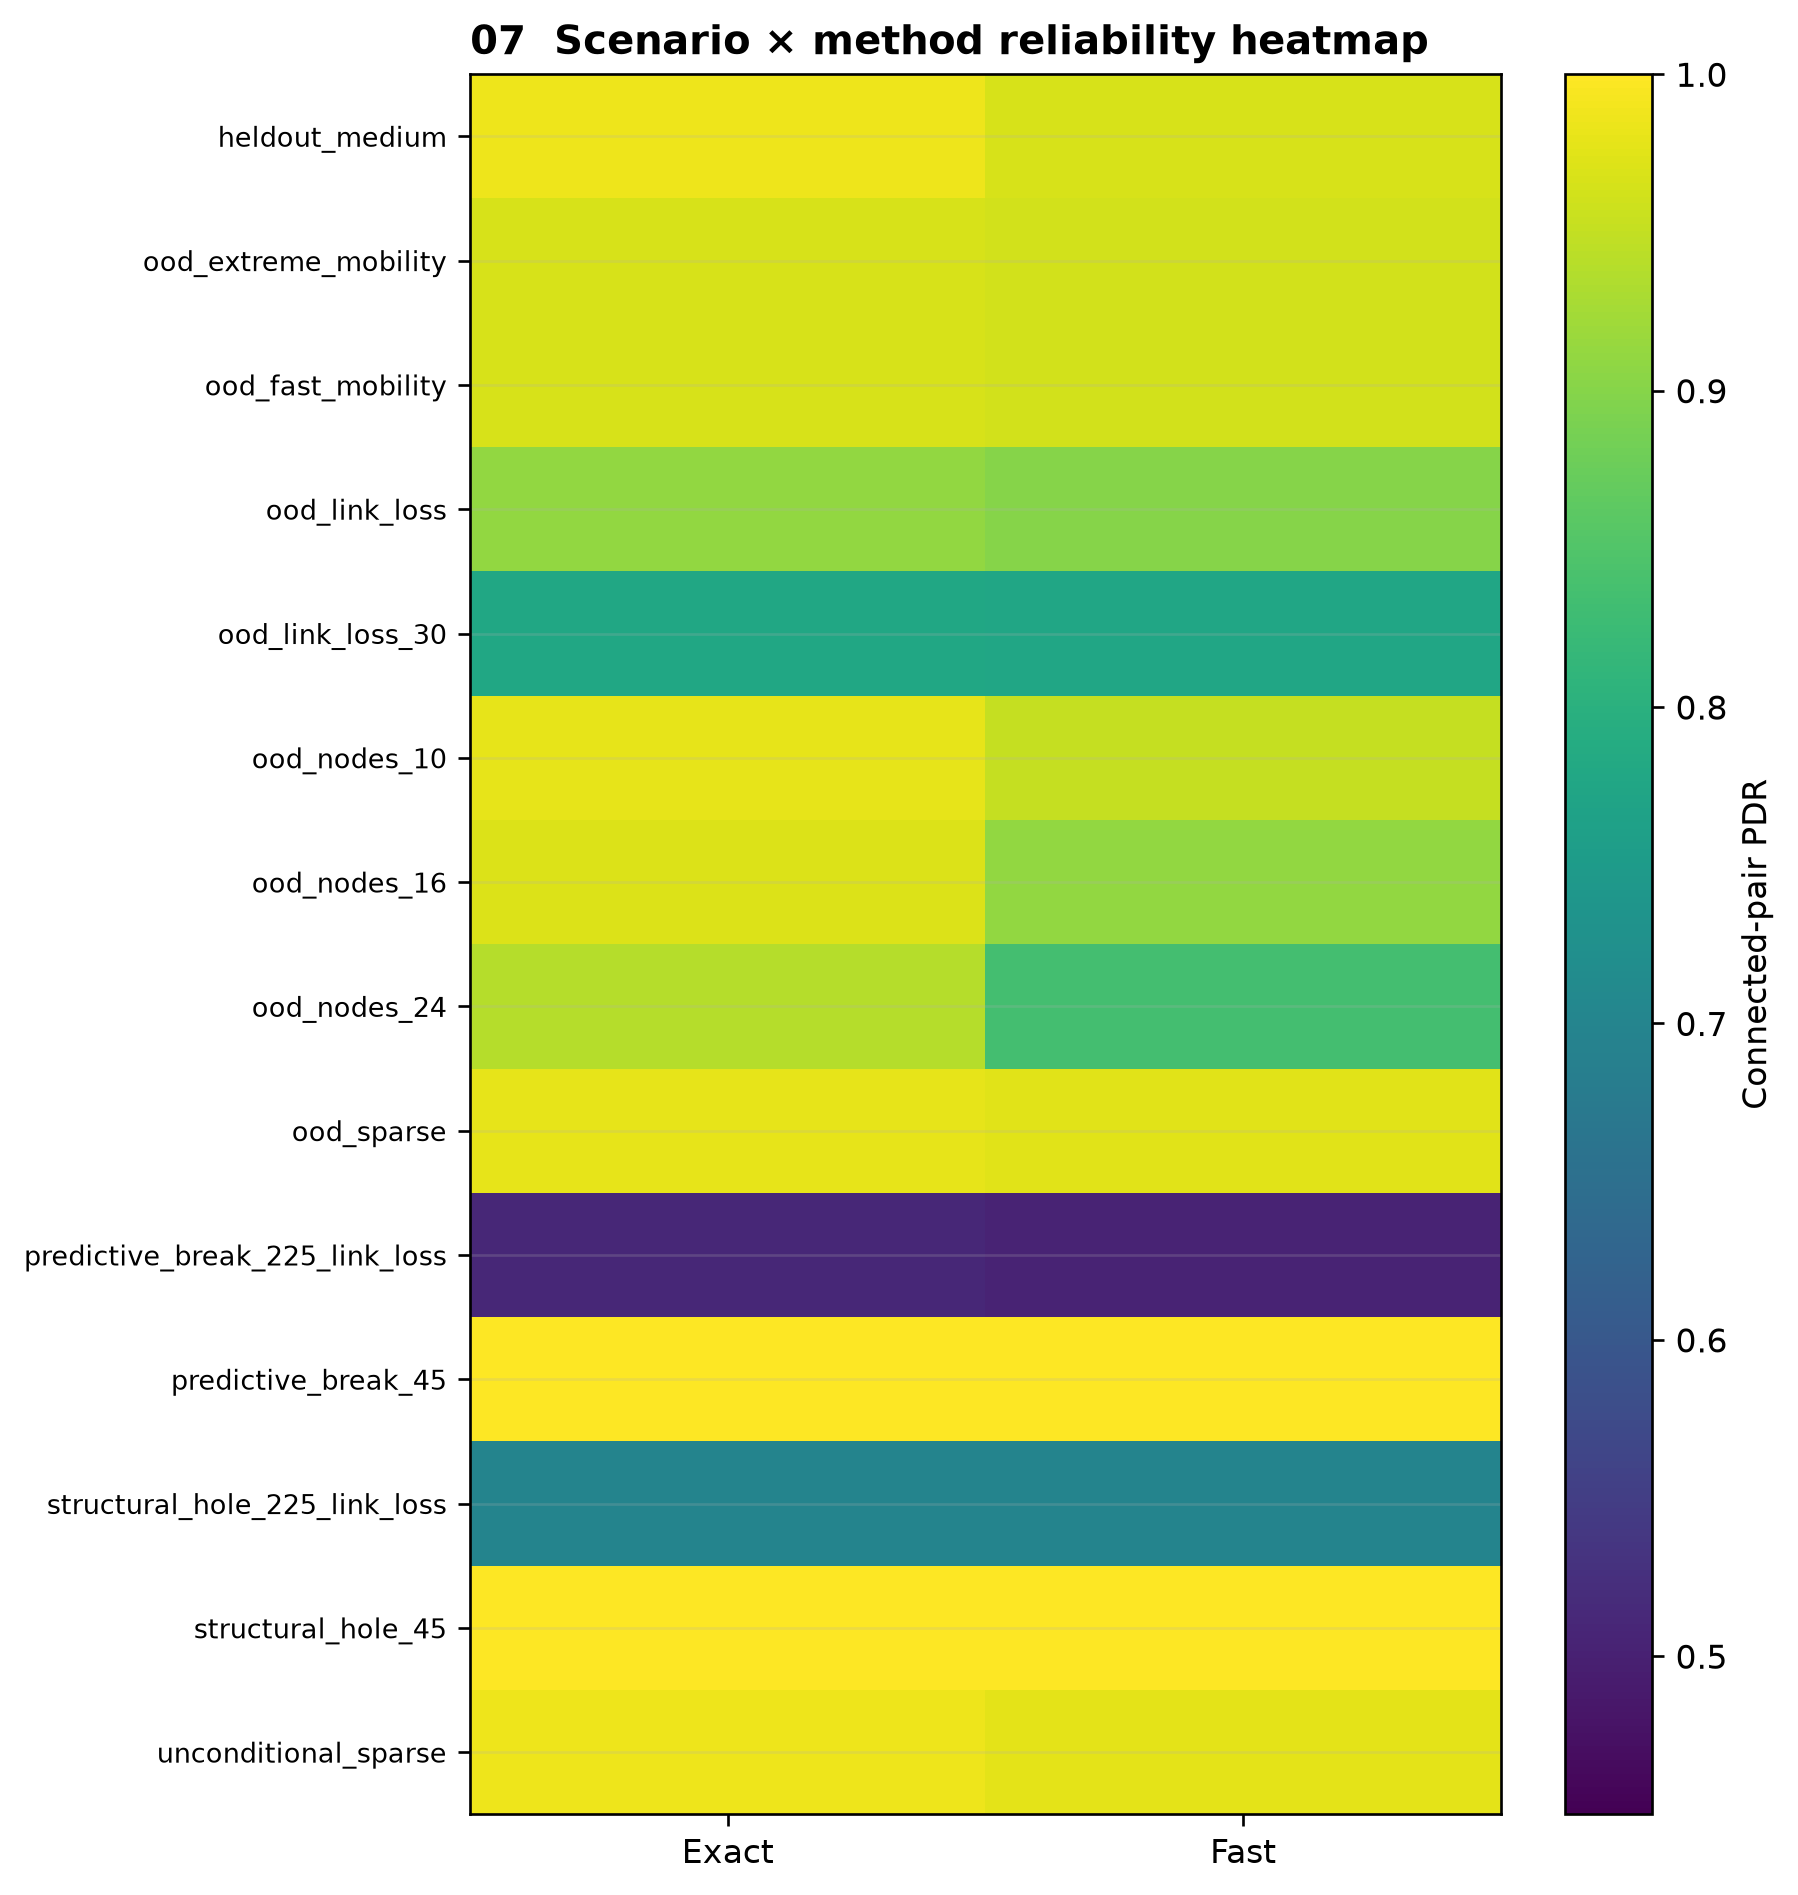
\includegraphics[width=\textwidth]{supplementary_figures/07_reliability_heatmap.png}
\caption{Five-seed scenario-level reliability. The heatmap localizes both predictive recovery and the node-scale or link-loss conditions in which approximations degrade.}
\label{fig:heatmap}
\end{figure*}

The three node-count-shift cases provide a limited generalization test, not a scalability proof. The full graph teacher is absent online, but the local tensor size still depends on the maximum candidate capacity and neighborhood representation. Larger swarms with higher local degree, realistic radio interference, and multiple concurrent flows require separate validation.

\subsection{Ablation Evidence}

Figure~\ref{fig:ablation} reports the seed-level contribution analysis. Removing the switch, relying on the predictive prior alone, or using the geographic-residual predecessor changes different scenario families. The result supports the architectural interpretation: global-to-local distillation supplies a capable normal policy, predictive features offer recovery information, and the calibrated switch prevents always-on predictive behavior from replacing safe nominal decisions indiscriminately.

\begin{figure*}[t]
\centering
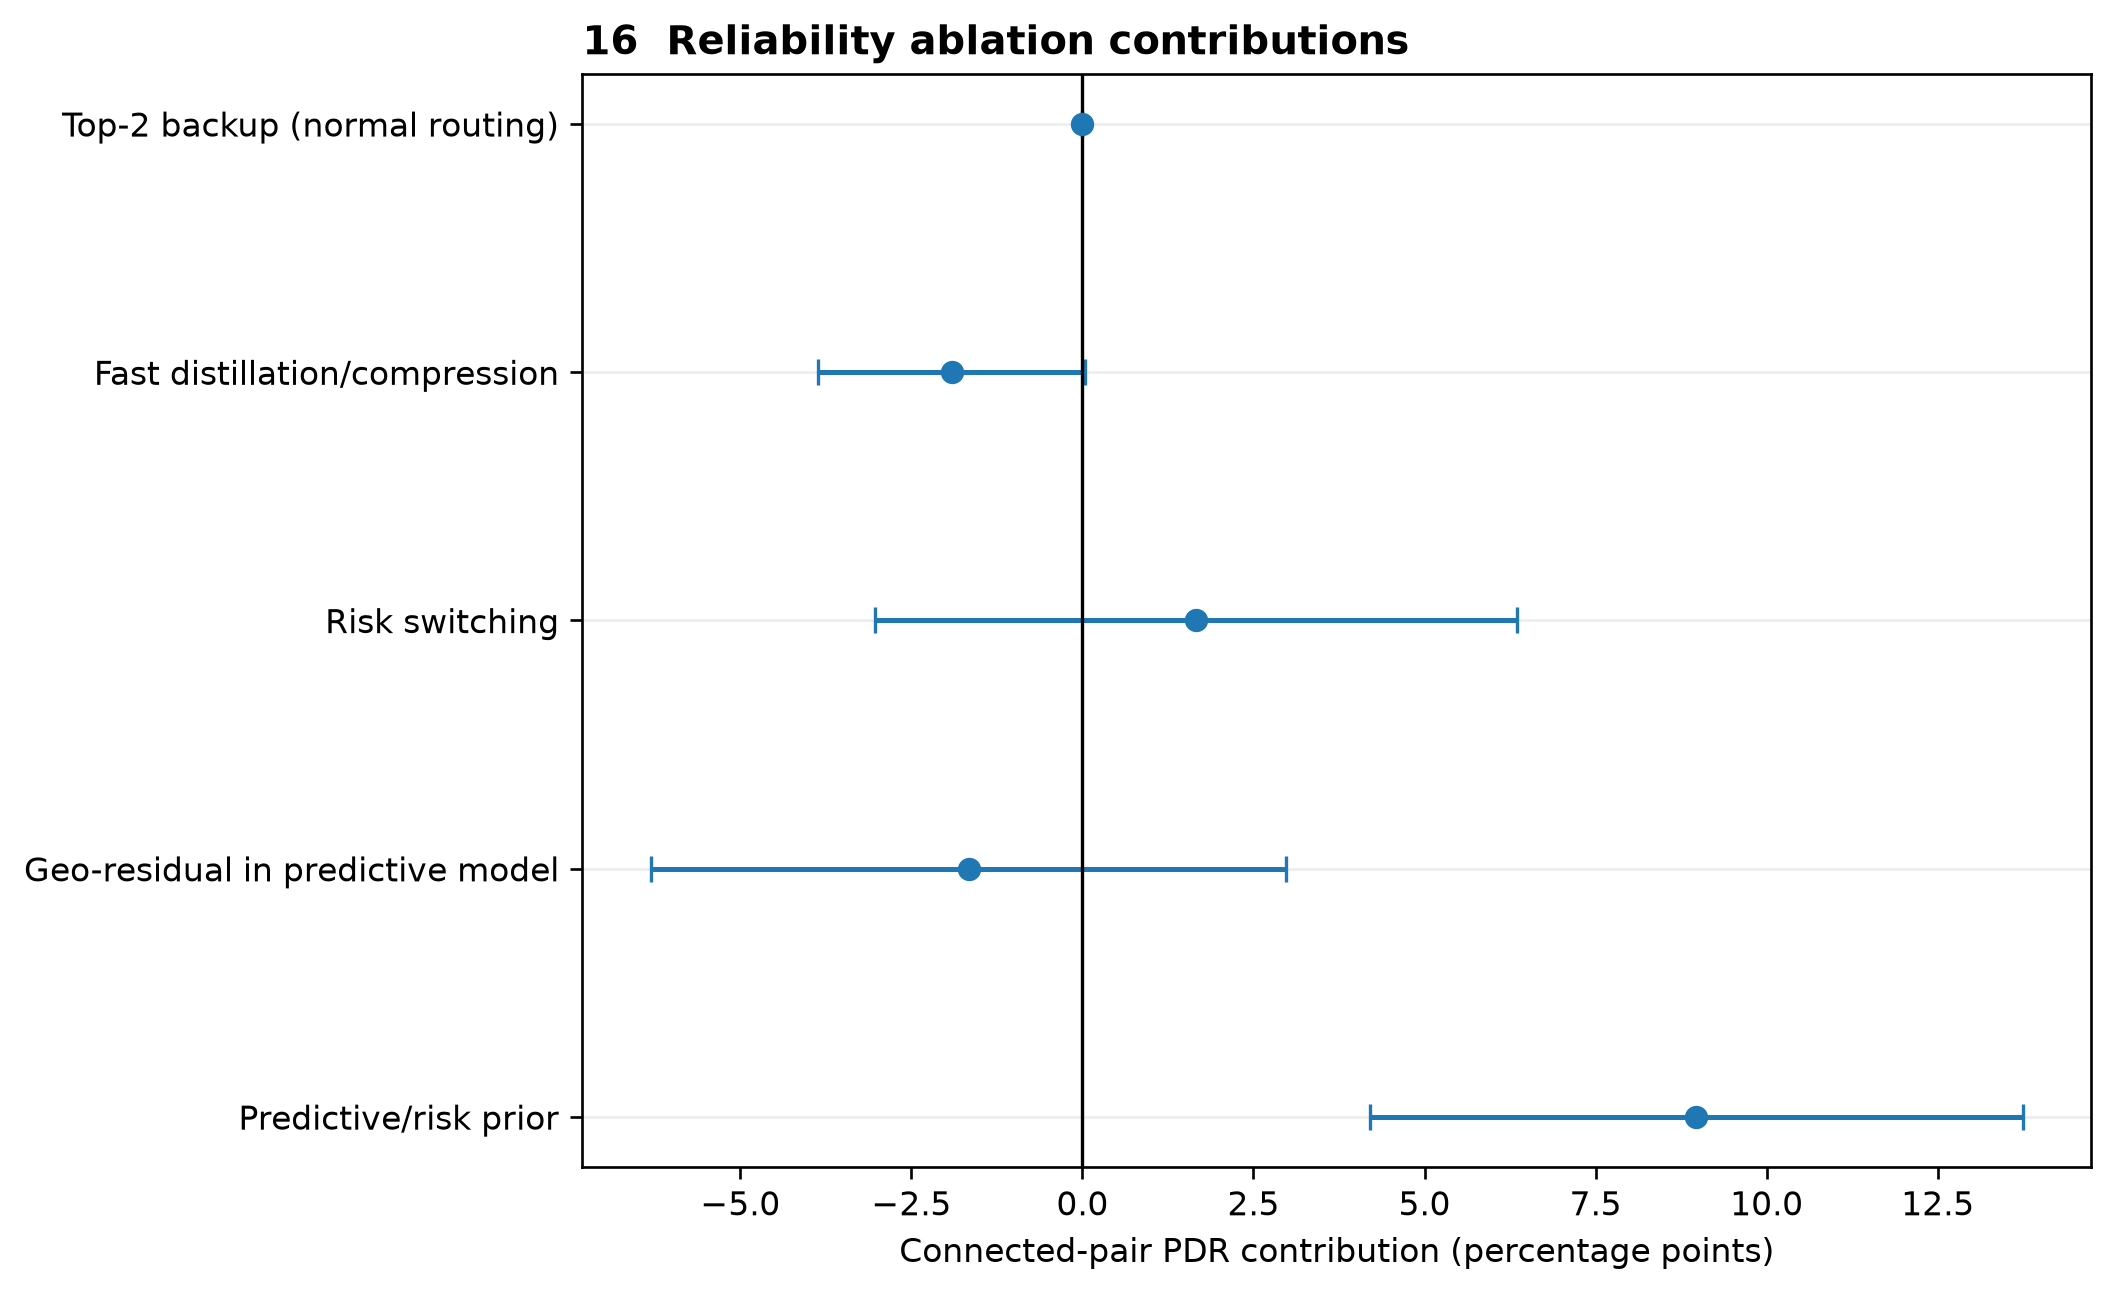
\includegraphics[width=0.92\textwidth]{supplementary_figures/16_ablation_contribution.png}
\caption{Directional component contributions with five-seed 95\% intervals. Positive values favor the complete Exact policy under the metric's preferred direction.}
\label{fig:ablation}
\end{figure*}

The project history includes additional negative interventions: increasing the Fast hidden dimension from 32 to 48 worsened the 24-node OOD case; density-augmented distillation improved node-count cases but introduced seed-specific predictive-break failures; switch recalibration under stochastic loss did not change the limiting outcome; and retraining the predictive student on that loss family reproduced the same failure pattern. These results are not promoted as separate contributions, but they constrain the explanation and motivate worst-scenario reweighting and action-space shielding.

\subsection{Exact Fusion and Batch-One Decision Latency}

Table~\ref{tab:latency} reports the same-session A100 results. The fused Exact CUDA p95 is 5.836 ms, compared with 10.004 ms for legacy repeated execution: a 41.66\% reduction. On the Colab host CPU, the corresponding values are 2.208 and 3.775 ms, a 41.51\% reduction. The exact policy result is unchanged because the speedup removes duplicate evaluation rather than changing a branch.

\begin{table*}[t]
\caption{Same-session batch-one end-to-end decision latency. Values are means of five seed-specific statistics; paired p95 change is relative to Exact and positive means faster.}
\label{tab:latency}\centering\scriptsize
\begin{tabularx}{\textwidth}{llYYYYY}
\toprule
Variant & Device & Mean (ms) & p50 & p95 & p99 & p95 change \\
\midrule
Exact fused & CPU & 2.168 & 2.161 & 2.208 & 2.344 & reference \\
Early Exit & CPU & 2.366 & 2.356 & 2.427 & 2.581 & $-9.90\%$ \\
Fast single pass & CPU & 0.812 & 0.814 & 0.847 & 0.927 & $+61.66\%$ \\
Fast + Top-2 & CPU & 0.853 & 0.852 & 0.881 & 0.933 & $+60.11\%$ \\
Buffered Exact & CPU & 2.187 & 2.179 & 2.244 & 2.370 & $-1.62\%$ \\
Legacy repeated & CPU & 3.698 & 3.687 & 3.775 & 3.935 & $-70.97\%$ \\
\midrule
Exact fused & CUDA & 5.671 & 5.648 & 5.836 & 6.101 & reference \\
Early Exit & CUDA & 6.198 & 6.172 & 6.386 & 6.663 & $-9.42\%$ \\
Fast single pass & CUDA & 1.957 & 1.950 & 2.005 & 2.120 & $+65.65\%$ \\
Fast + Top-2 & CUDA & 2.040 & 2.032 & 2.092 & 2.183 & $+64.16\%$ \\
Buffered Exact & CUDA & 5.626 & 5.602 & 5.788 & 6.020 & $+0.83\%$ \\
Legacy repeated & CUDA & 9.741 & 9.706 & 10.004 & 10.376 & $-71.43\%$ \\
\bottomrule
\end{tabularx}
\end{table*}

\begin{figure*}[t]
\centering
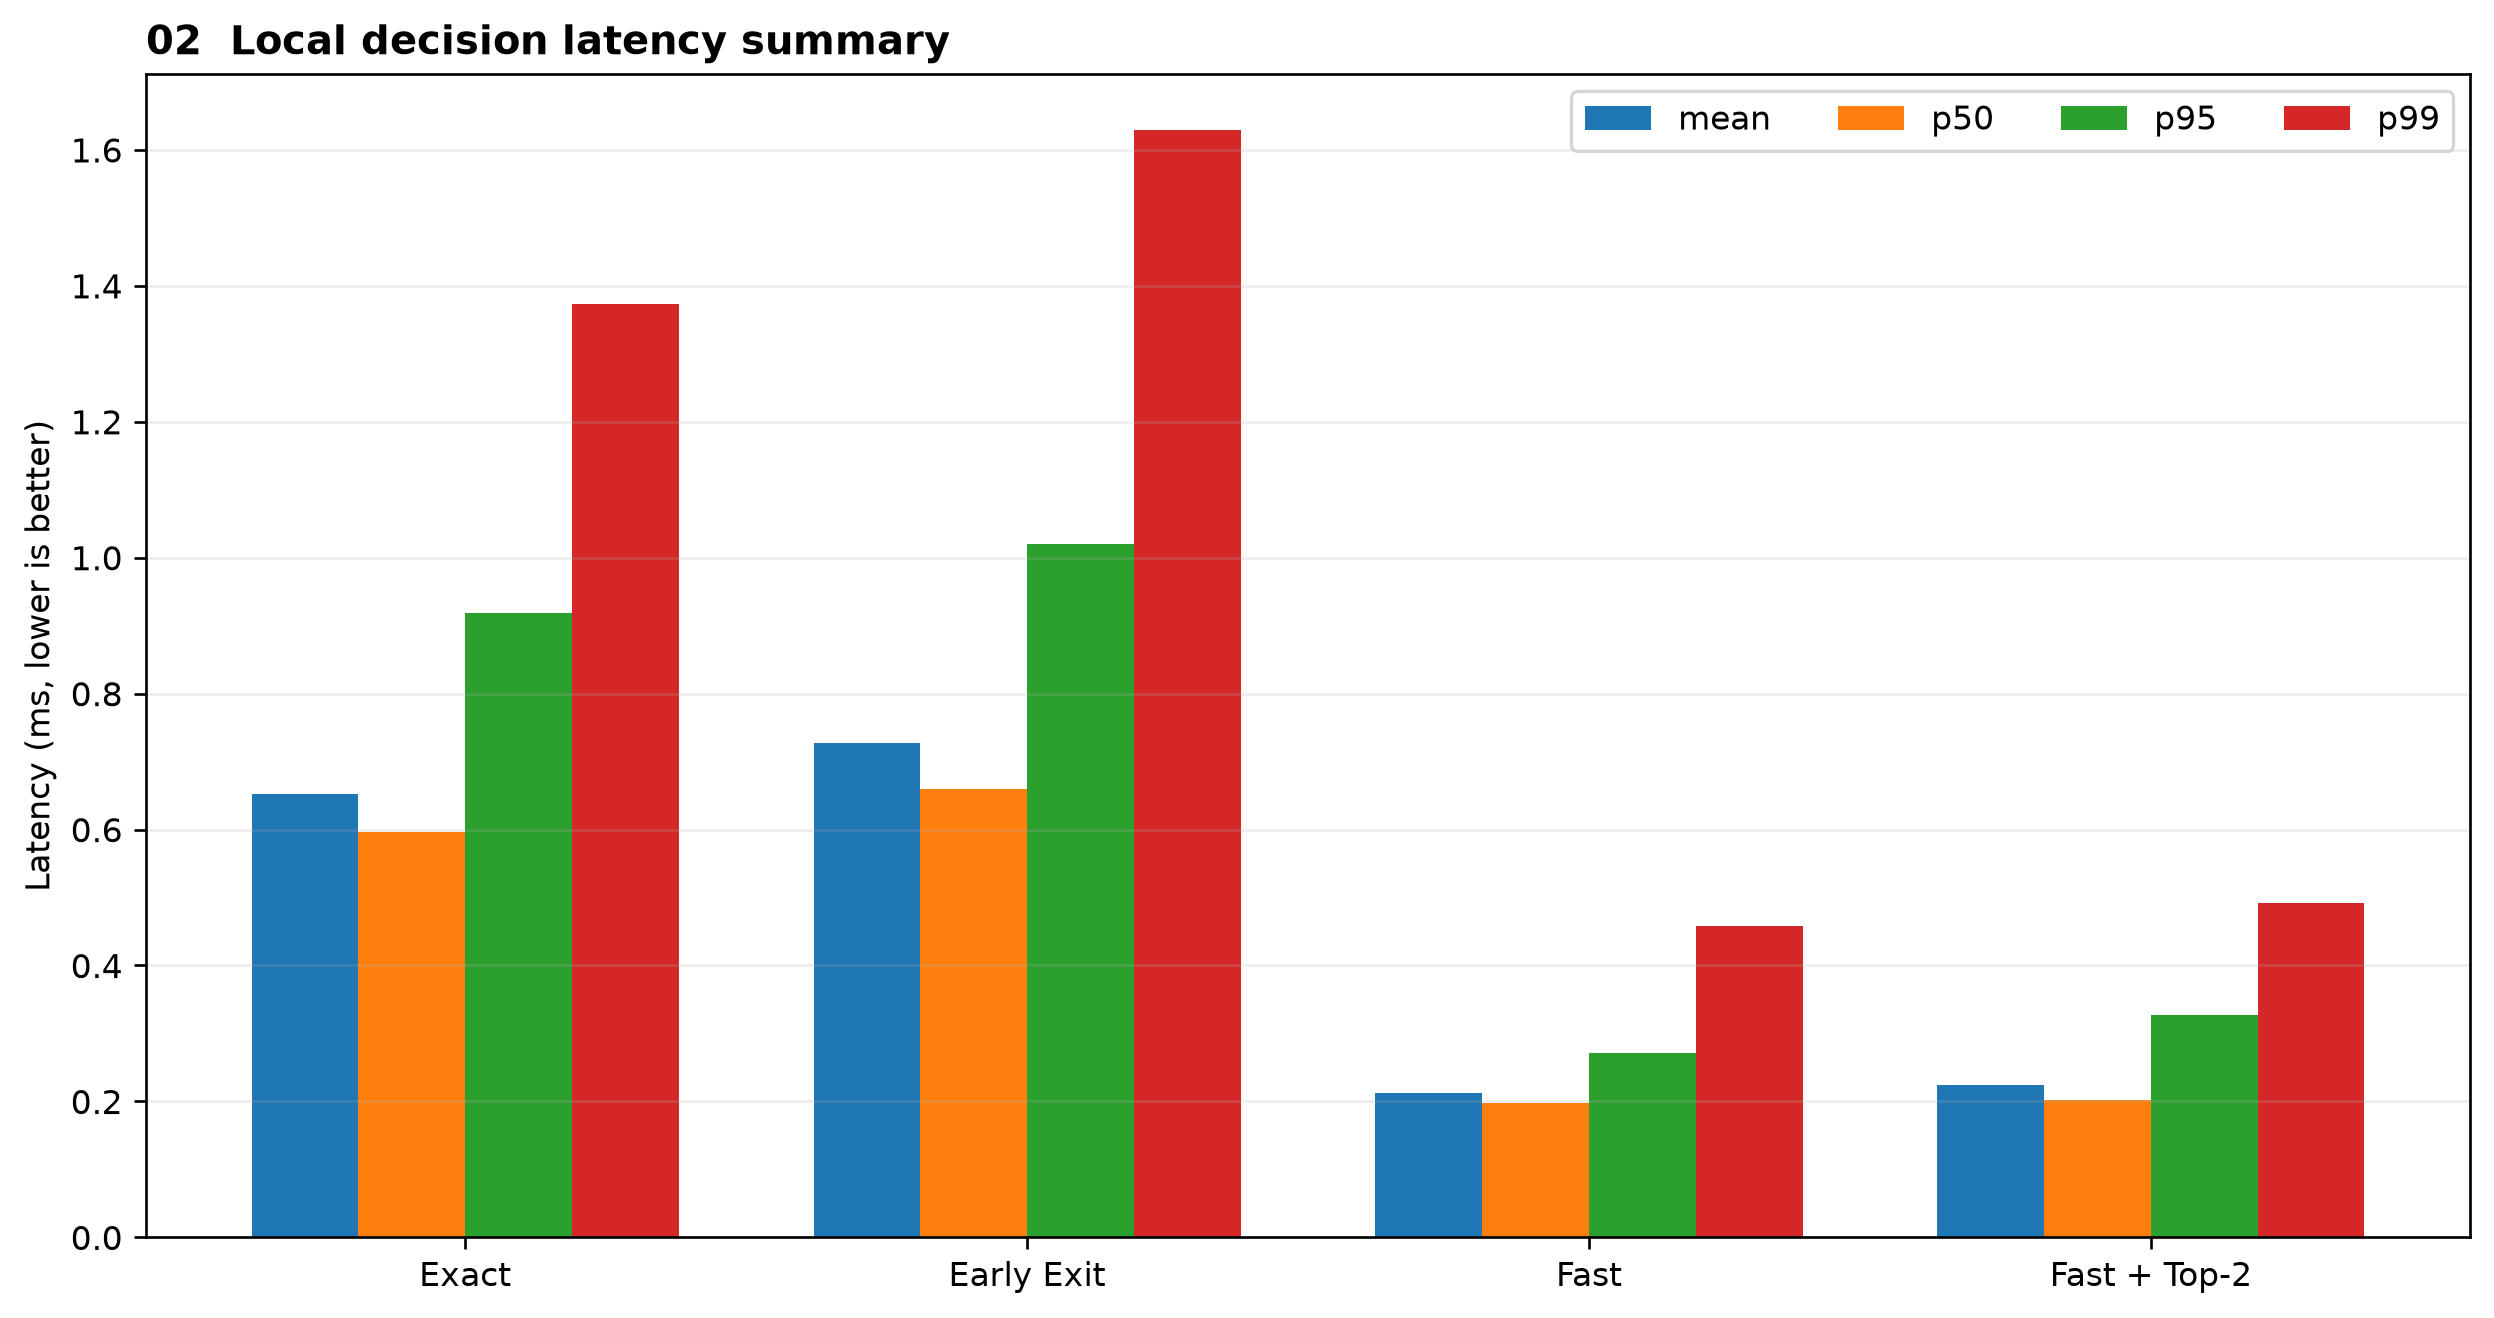
\includegraphics[width=0.92\textwidth]{supplementary_figures/02_latency_summary.png}
\caption{Latency summary across the verified implementations. The low Fast latency must be read together with its reliability failure.}
\label{fig:latencysummary}
\end{figure*}

The paired CUDA p95 reduction for Buffered Exact is only 0.83\% (95\% $t$ CI 0.21--1.44); it is classified as ``hold'' because the effect is small and is negative on CPU. Early Exit is 9.42\% slower on CUDA (CI $-10.62$ to $-8.22$). Figure~\ref{fig:forest} shows the uncertainty and direction of these effects.

\begin{figure*}[t]
\centering
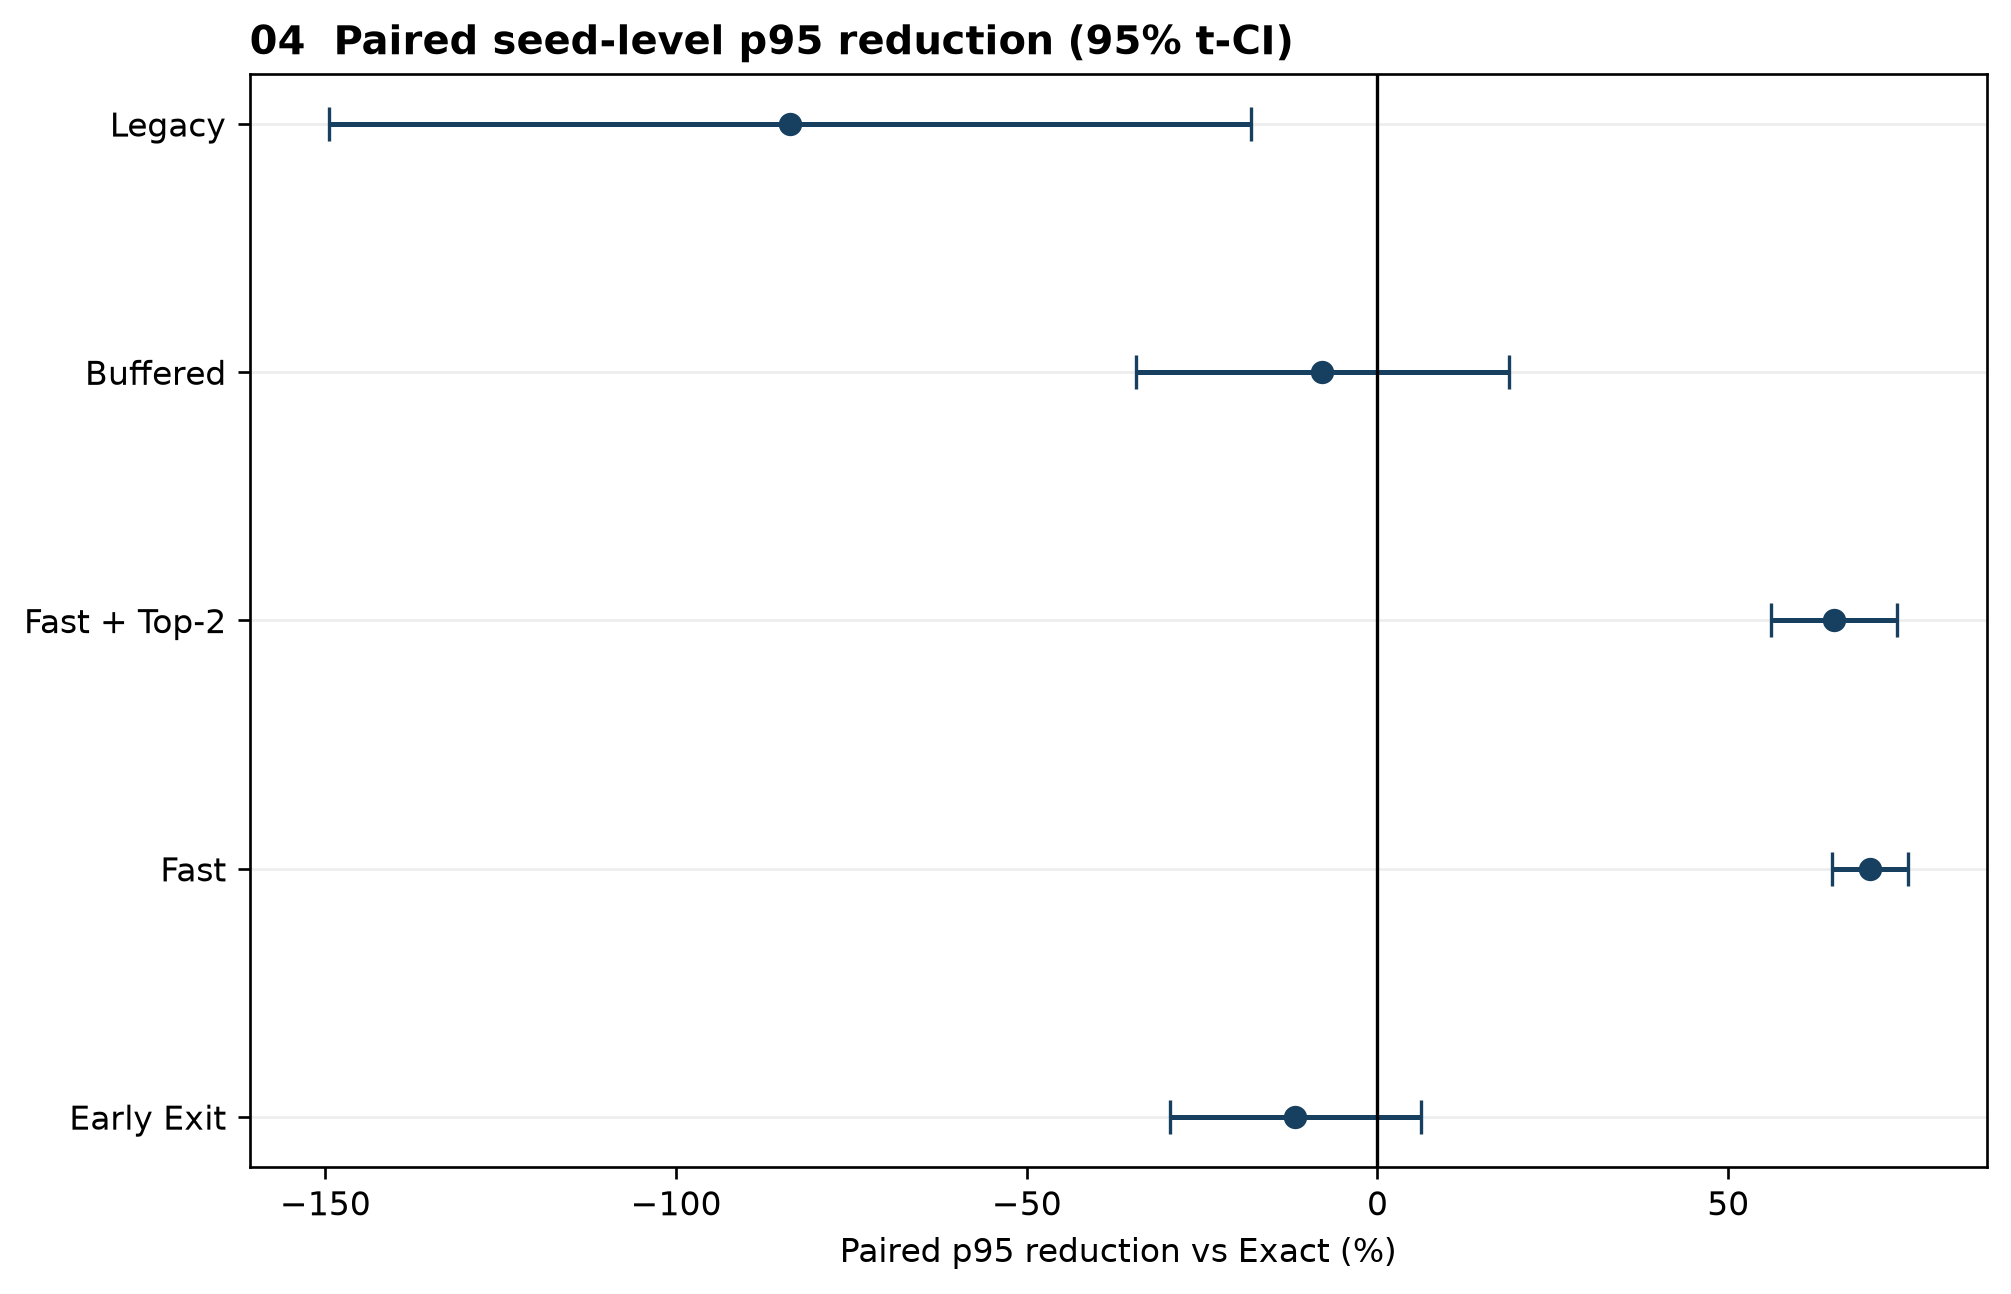
\includegraphics[width=0.90\textwidth]{supplementary_figures/04_latency_forest.png}
\caption{Paired p95 latency effects versus Exact. Positive values favor the candidate. Intervals are based on five matched checkpoints, not on 10,000 pseudo-independent individual calls.}
\label{fig:forest}
\end{figure*}

\subsection{Why CUDA Is Slower Than the CPU}

Exact is 62.16\% faster on the A100-session host CPU than on CUDA at p95 (2.208 versus 5.836 ms). This result is consistent with a fine-grained batch-one workload. The model has small matrix operations, while each CUDA decision launches many kernels, constructs or transfers small tensors, and materializes scalar values for Python-side conditions and action extraction. The fixed launch and synchronization costs dominate the compute saved by parallel arithmetic.

Operator profiling supports this attribution. Across 30 Exact profiled calls, the local-scalar materialization operator occurs 1,050 times and is paired with 1,050 device-to-host copies. Early Exit increases these counts to 1,140; Fast reduces them to 300. The profiler cannot apportion the complete synchronized p95, but it identifies a plausible synchronization mechanism and explains why Python conditional execution does not satisfy $T_g<p_{\mathrm{skip}}T_P$.

Figure~\ref{fig:device} shows the device comparison. It does not imply that every CPU is faster than every embedded GPU. Deployment must be remeasured on the target flight computer, preferably including power and forwarding-table update time.

\begin{figure*}[t]
\centering
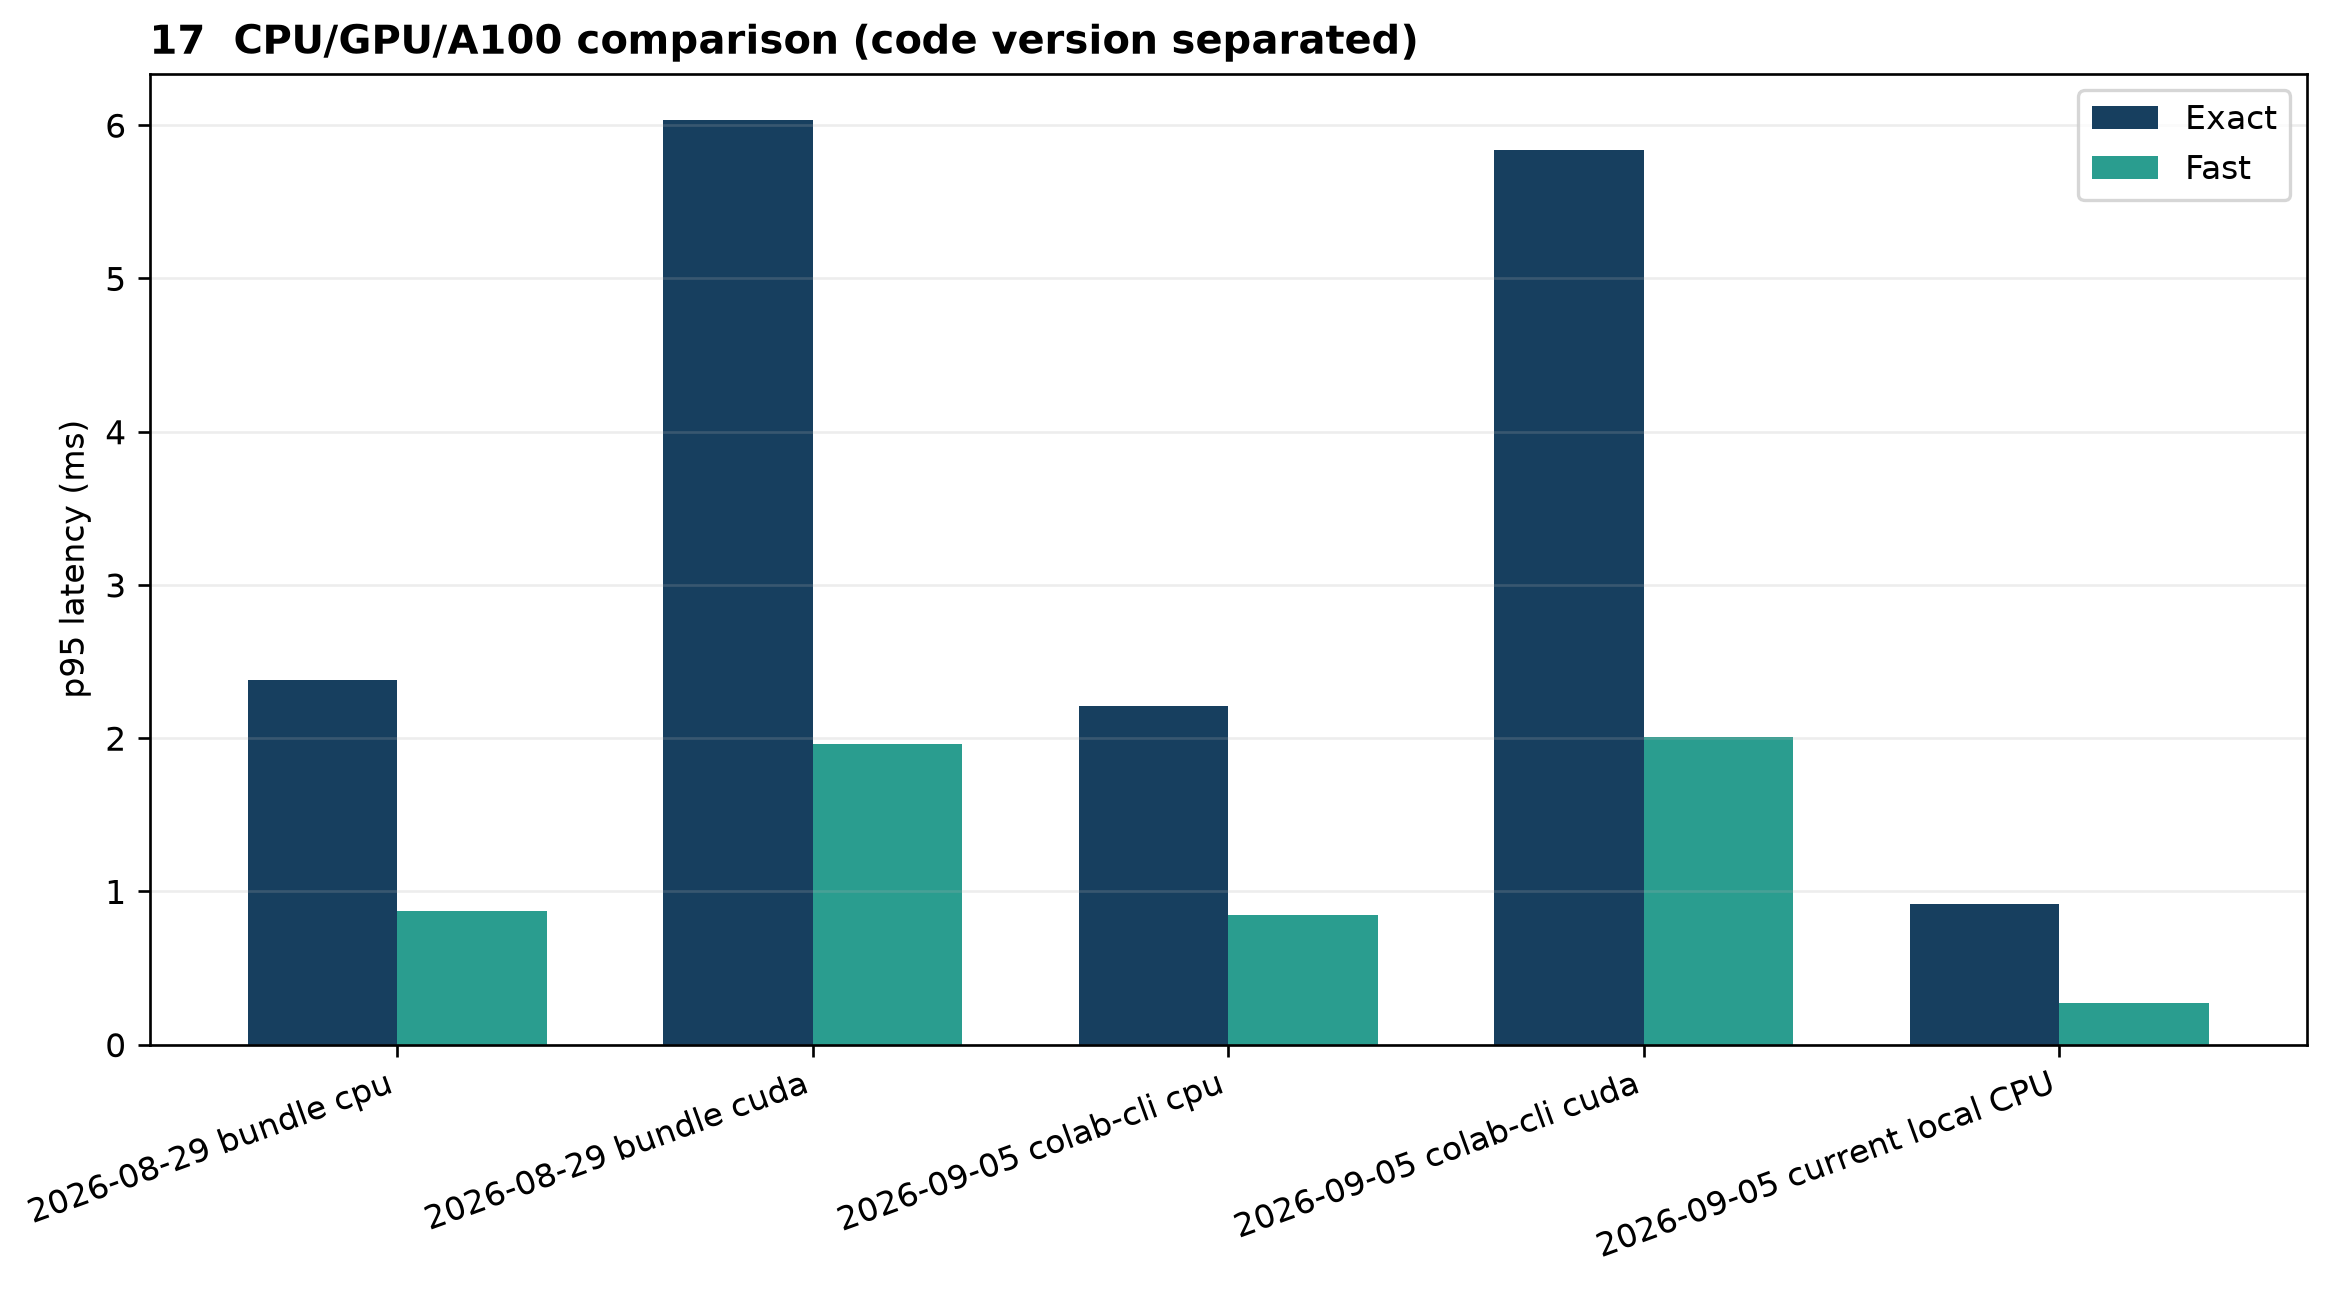
\includegraphics[width=0.92\textwidth]{supplementary_figures/17_device_comparison.png}
\caption{CPU and CUDA decision latency in the verified A100 session, with an older bundle retained only as an independent reproducibility reference.}
\label{fig:device}
\end{figure*}

\subsection{Why Fast Does Not Replace Exact}

\FastSG{} reduces CUDA p95 to 2.005 ms, 65.65\% below Exact, but connected PDR decreases from 0.90529 to 0.88720. The directional paired change is $-0.01809$ with 95\% CI $[-0.03606,-0.00011]$, below the predeclared $-0.005$ non-inferiority floor. Deadline ratio decreases by 0.02264 with CI $[-0.04625,0.00096]$; successful p95 delay and energy proxy also worsen. The compact model is therefore a latency--quality research candidate, not the final method.

\begin{figure*}[t]
\centering
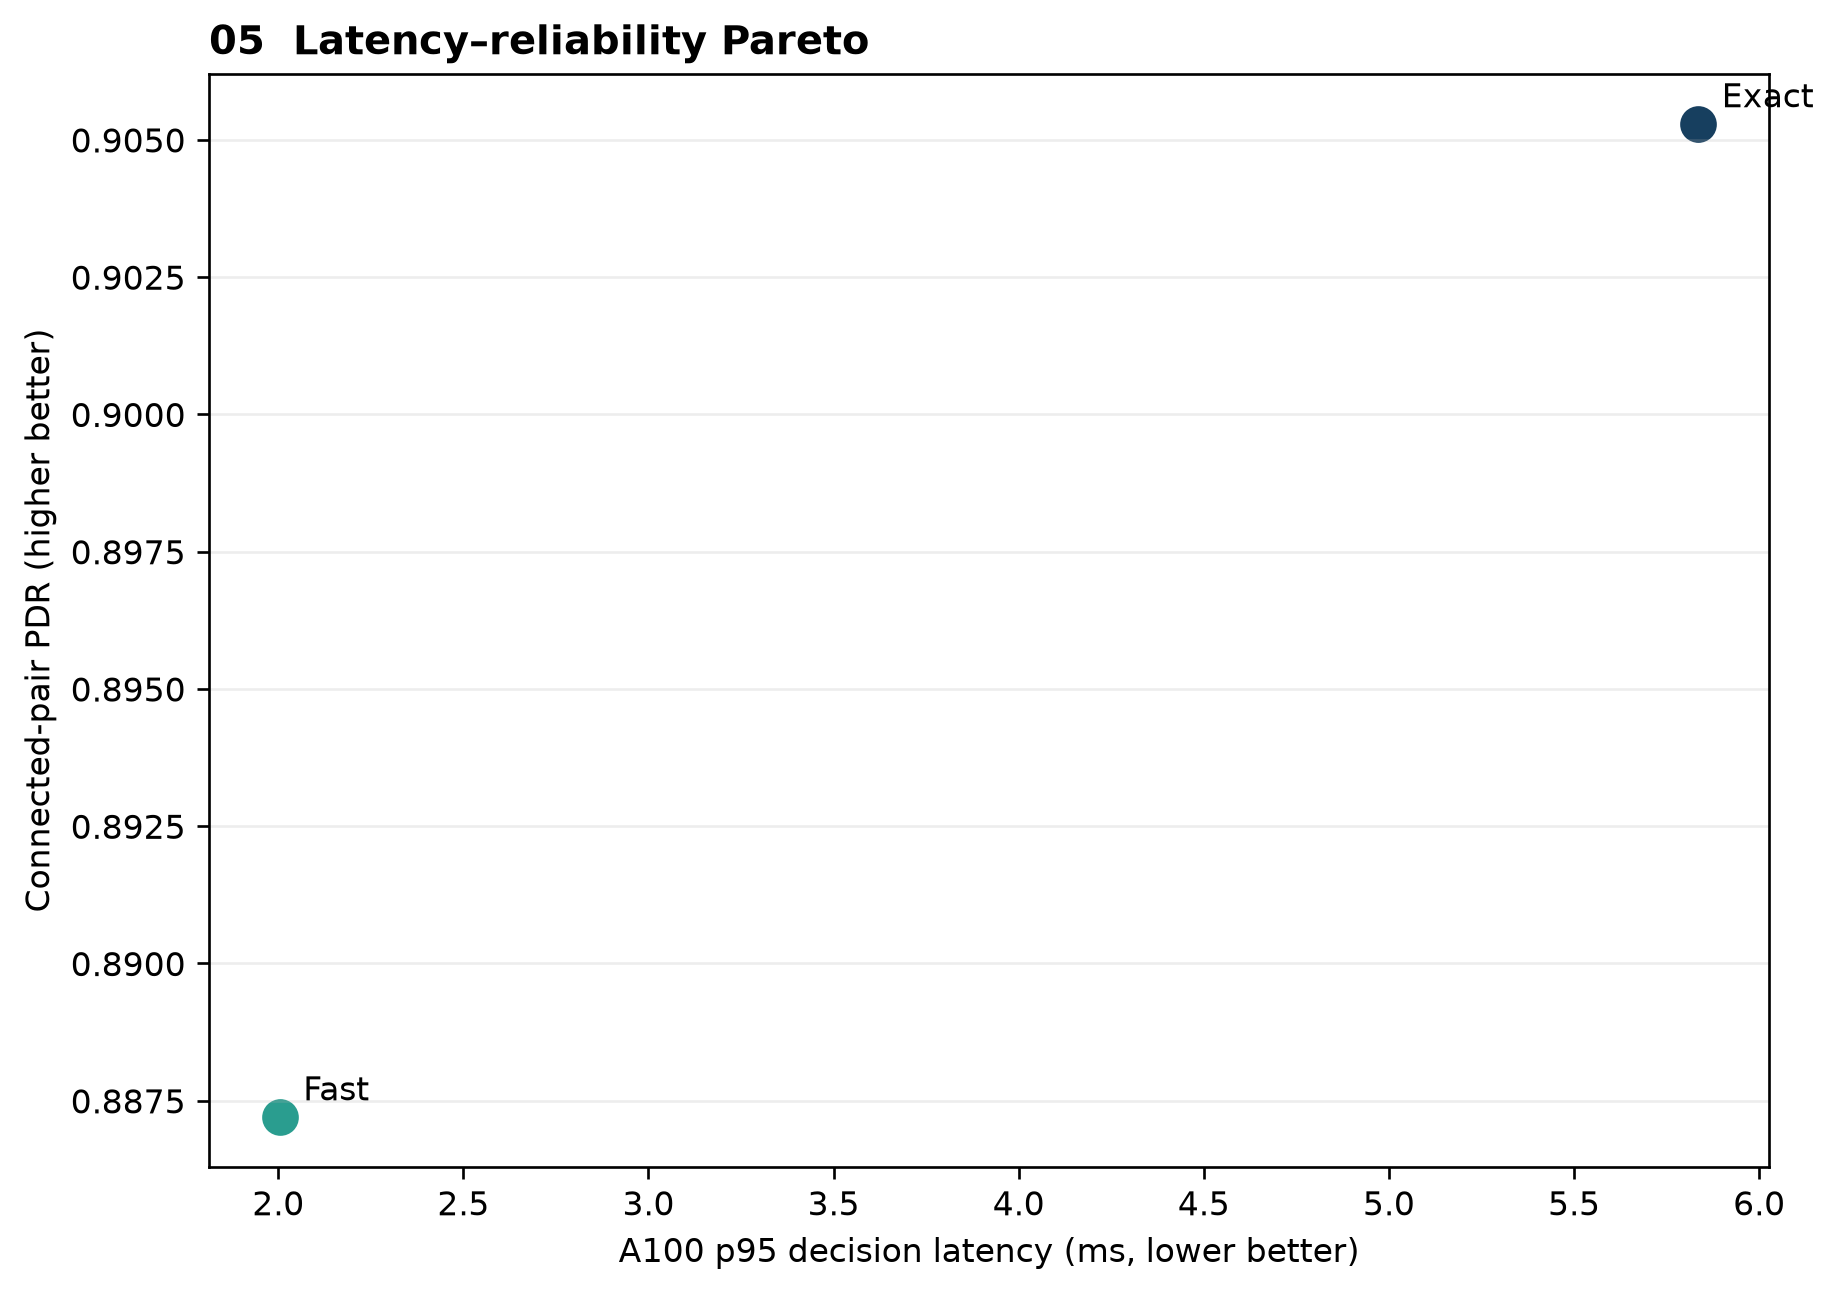
\includegraphics[width=0.90\textwidth]{supplementary_figures/05_pareto_connected_pair_pdr.png}
\caption{A100 p95 decision latency versus connected-pair PDR. The upper-left region is preferred; Exact and Fast represent distinct quality--latency choices.}
\label{fig:pareto}
\end{figure*}

\begin{figure*}[t]
\centering
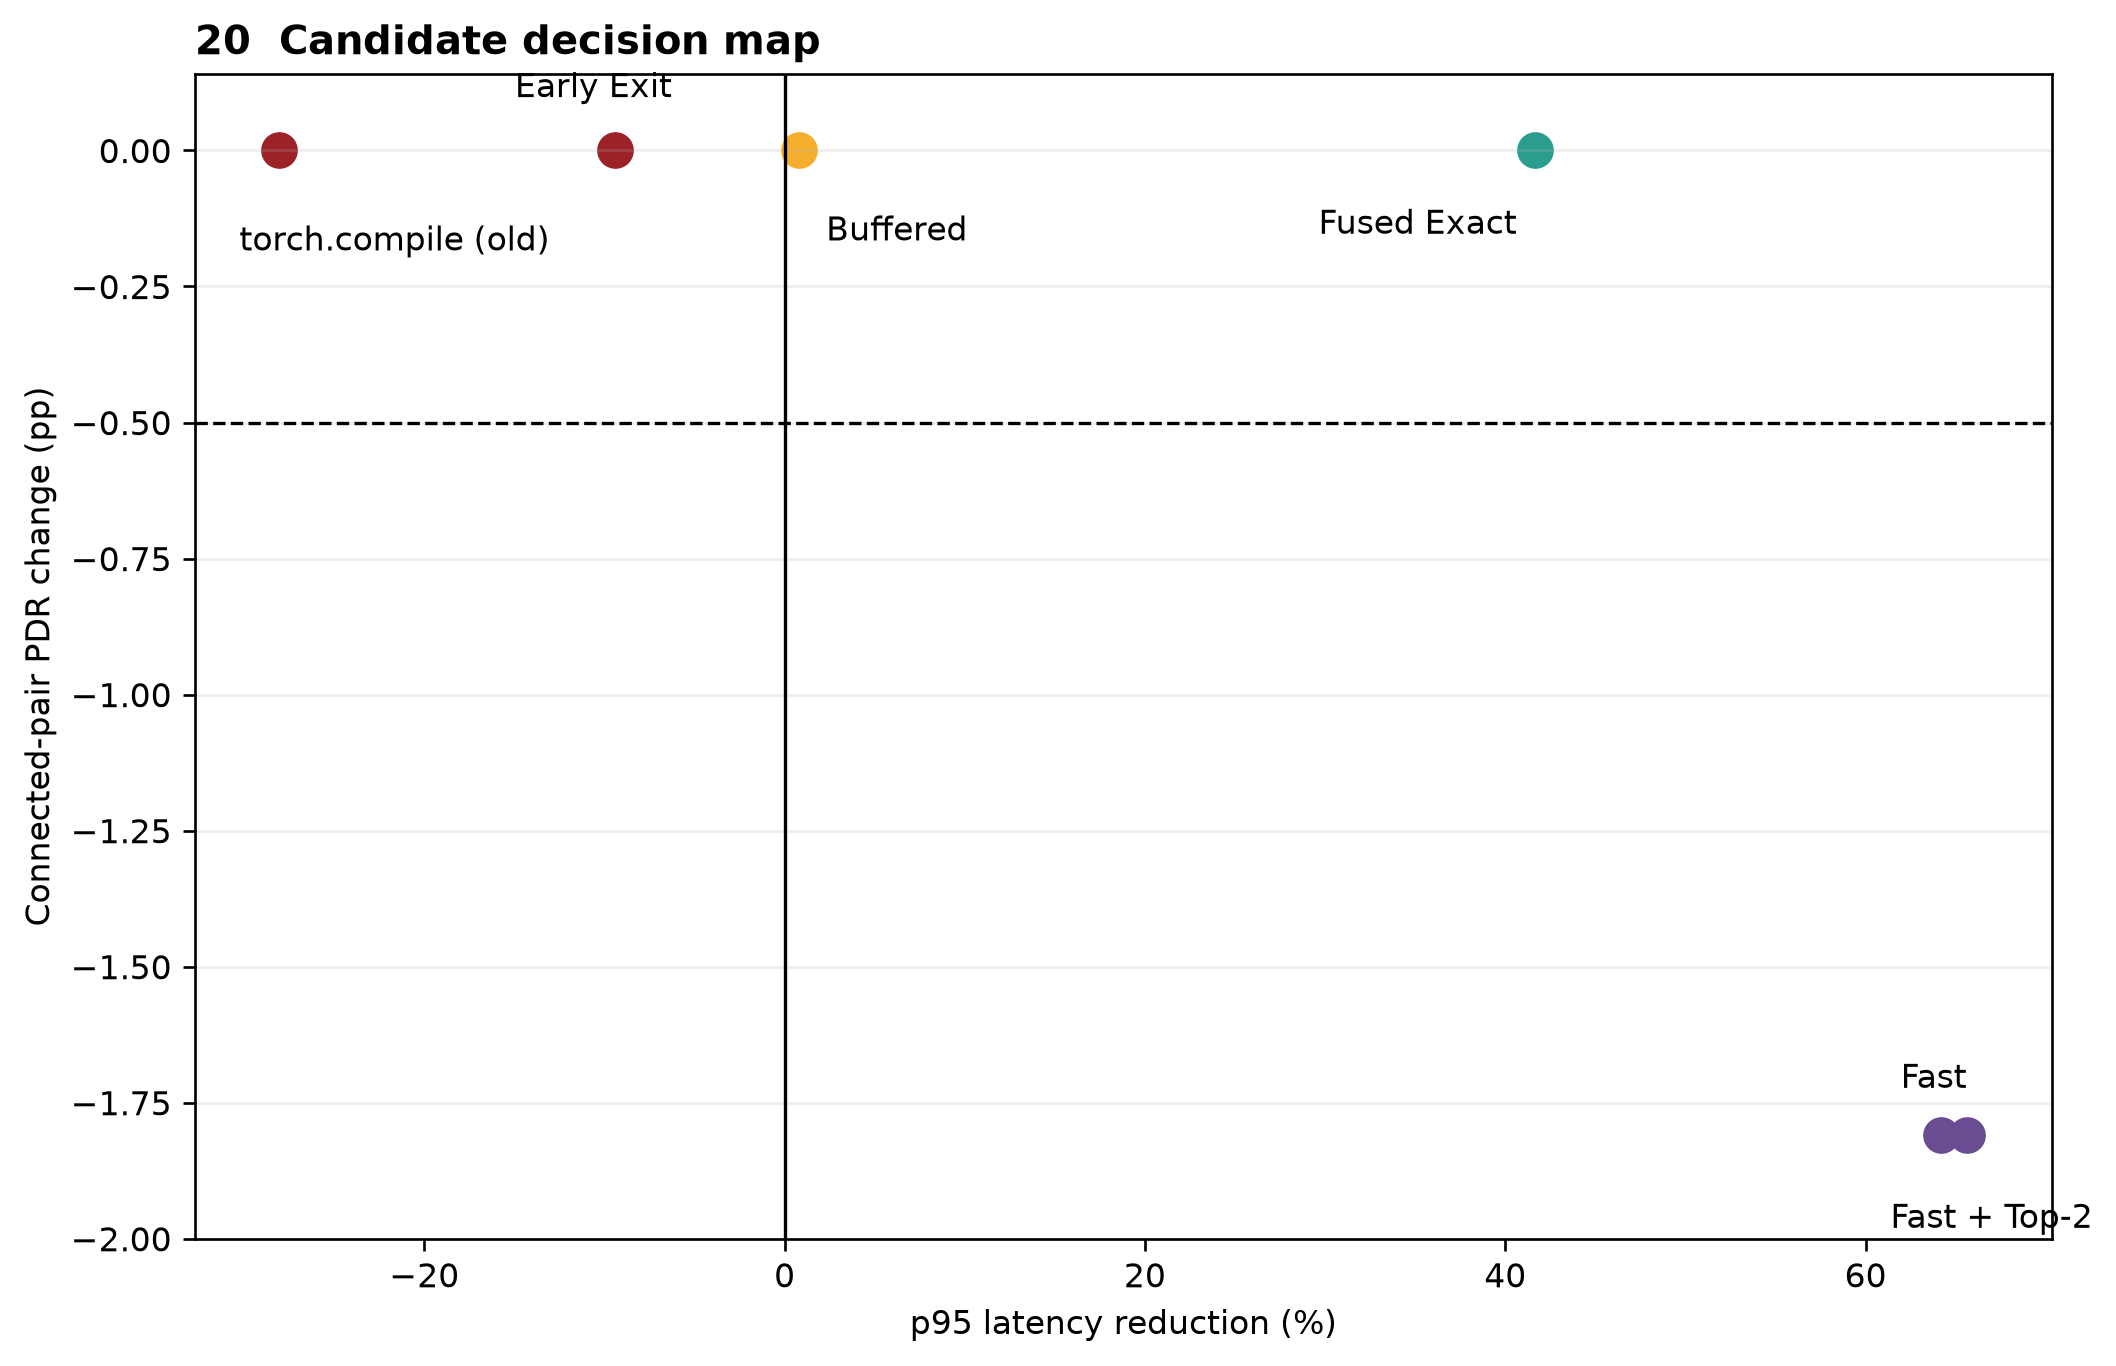
\includegraphics[width=0.92\textwidth]{supplementary_figures/20_failed_candidate_tradeoff.png}
\caption{Decision record for optimization candidates. Fused Exact is accepted because it preserves exact behavior; Fast fails reliability, and Python Early Exit fails latency.}
\label{fig:decision}
\end{figure*}

\subsection{Early-Exit Calibration as a Negative Result}

At a zero danger margin, Early Exit skips the predictive branch for 32,285 of 43,467 decisions (74.27\%) and produces no episode-trajectory mismatch over 14,000 paired episodes for the current checkpoints and scenarios. Positive margins increase the skip rate but cause action divergence. Figure~\ref{fig:gate} shows this empirical calibration boundary.

\begin{figure*}[t]
\centering
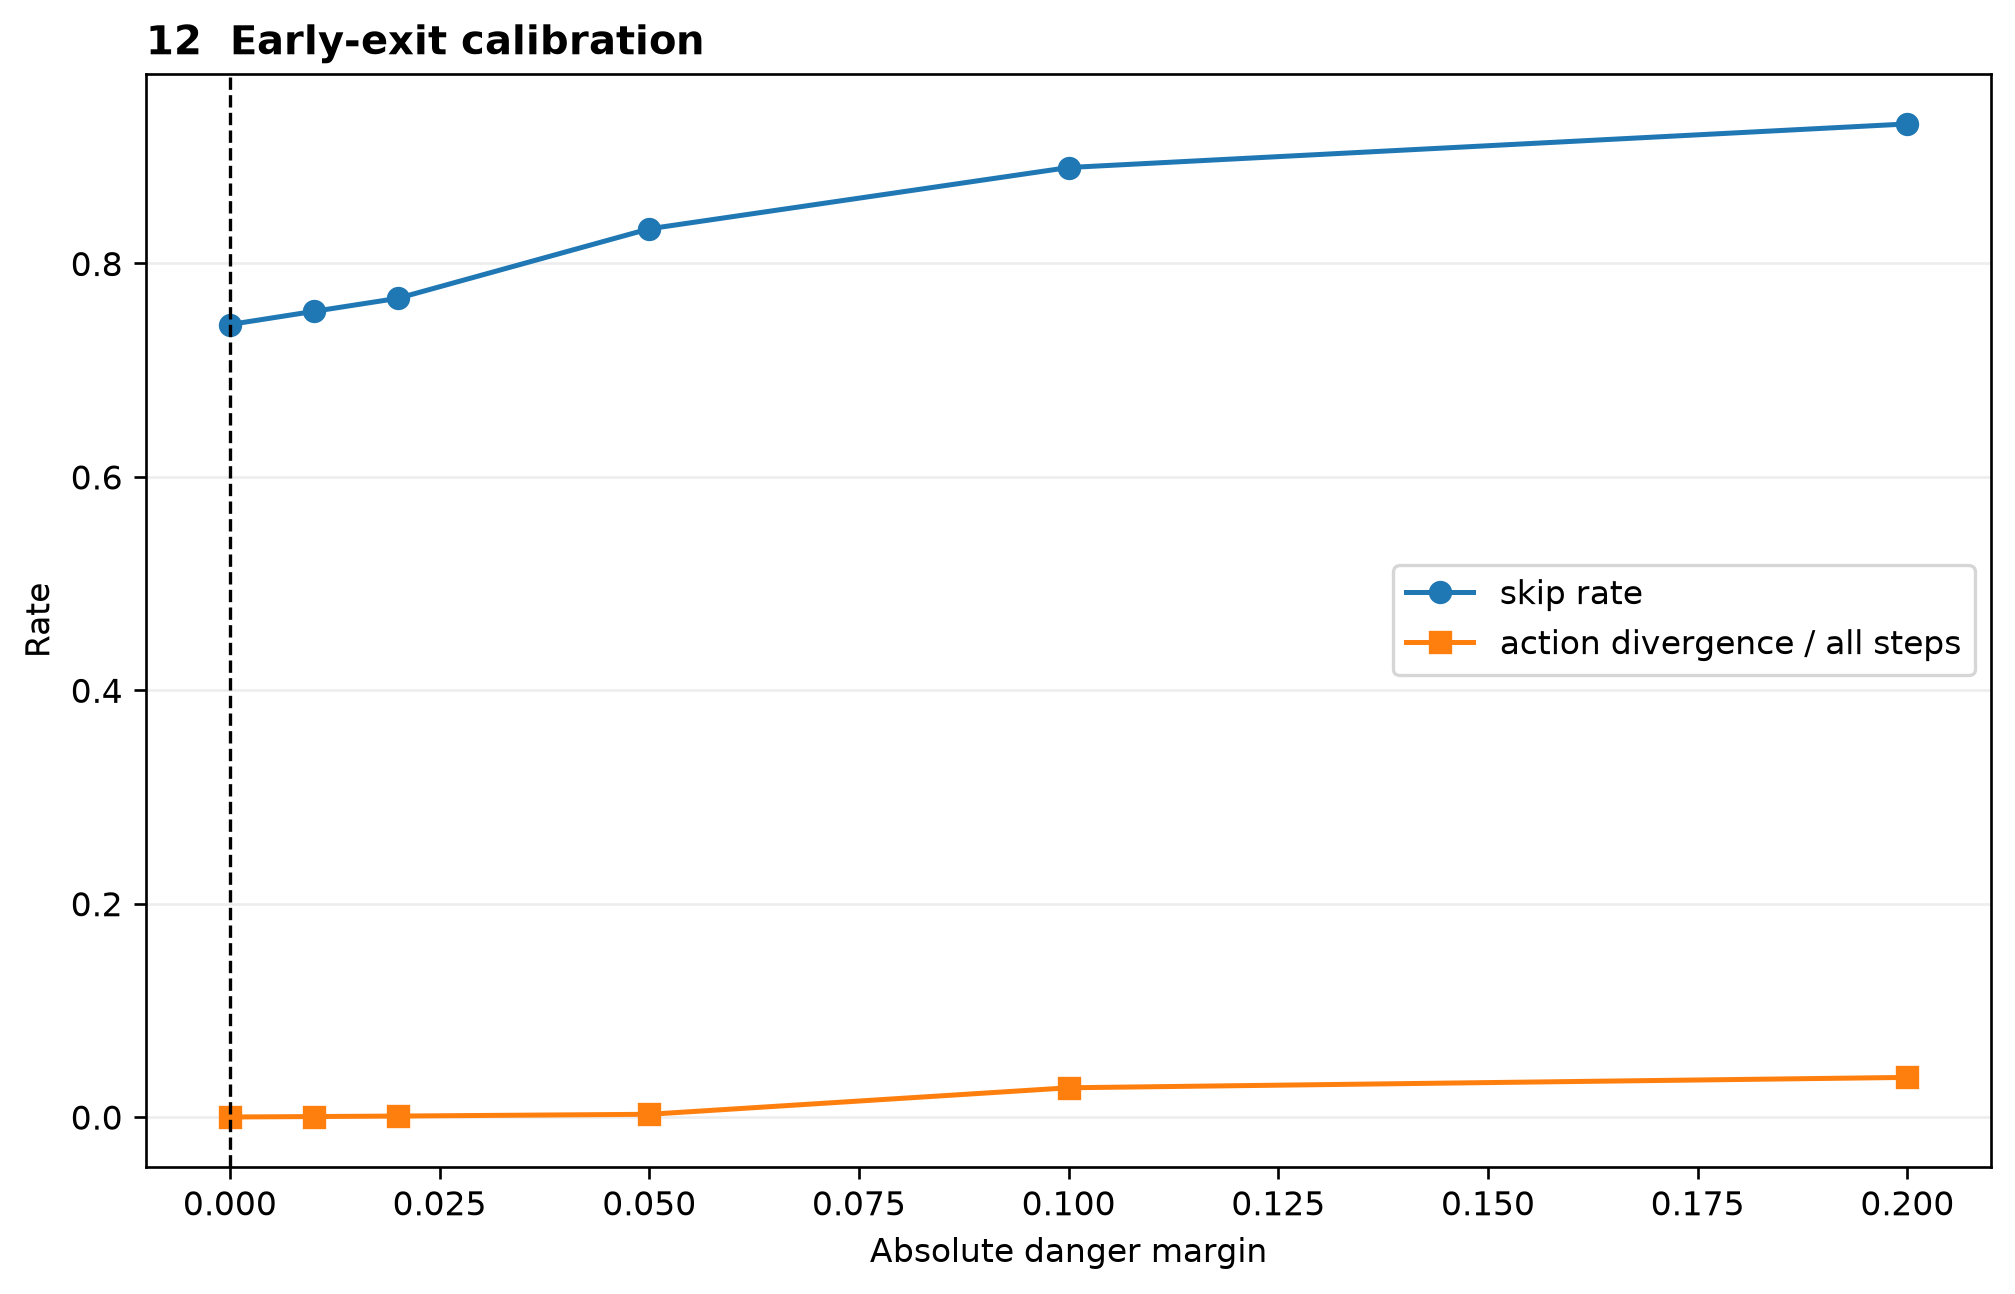
\includegraphics[width=0.88\textwidth]{supplementary_figures/12_gate_calibration.png}
\caption{Early-exit calibration. Zero observed divergence at margin zero is empirical evidence for the evaluated trajectories, not formal equivalence for unseen states.}
\label{fig:gate}
\end{figure*}

Despite the high skip rate, Early Exit is slower. Its Python branch requires scalar materialization and control flow before saving a small predictive multilayer perceptron call. This negative result rules out the naive ``high skip rate implies low latency'' argument and motivates a tensor-only conditional graph, such as a deployment-runtime conditional operator, for future work.

\section{Discussion}

\subsection{Answering the Research Questions}

First, the common-simulator evidence supports the strict-local architecture: Exact provides the strongest scenario-macro reliability and deadline delivery among the eight implementations, with paired advantages over the strongest adapted baseline. The claim is deliberately limited to the evaluated simulator, information contracts, and scenarios.

Second, recovery is not attributable to a single black-box network. The geographic prior stabilizes nominal forwarding, the distilled residual transfers global structural preference to local features, predictive risk exposes impending breaks, and the calibrated switch determines when the predictive prior should replace the nominal choice. The ablation and scenario heatmap show complementary roles and a remaining predictive-break-with-loss weakness.

Third, exact execution fusion materially reduces the avoidable portion of decision latency, but the remaining model is too fine-grained to benefit automatically from the A100 at batch one. Host-device synchronization and launch overhead are part of the routing system, not incidental benchmarking noise. For online packet routing, batching decisions can change the control semantics or add waiting delay; batch one is therefore the deployment-relevant primary measurement.

Fourth, neither Fast nor the tested Early Exit is an acceptable replacement. Fast wins the timer and loses the predeclared quality gate. Early Exit preserves observed trajectories at its conservative threshold but loses the timer. Fused Exact is the final \SG{} implementation because it is the only tested change that offers a large latency reduction relative to the duplicated legacy path without changing the policy.

\subsection{End-to-End Delay Versus Decision Latency}

Both quantities should be measured, but they answer different questions. Network end-to-end delay can be written schematically as
\begin{equation}
\begin{aligned}
T_{\mathrm{E2E}}=\sum_{h=1}^{H}\big(&T_{\mathrm{queue},h}+T_{\mathrm{MAC},h}
+T_{\mathrm{tx},h}\\
&{}+T_{\mathrm{prop},h}+T_{\mathrm{decision},h}
+T_{\mathrm{update},h}\big).
\end{aligned}
\end{equation}
The simulator's successful delay in steps captures the route-level effect of hop count, retries, and connectivity under its abstraction. The microbenchmark isolates observation-to-action software latency. A future hardware-in-the-loop evaluation should add routing-table update and real radio timing. Combining these terms into one unlabeled ``delay'' would make comparison with RoutePPO, RLFR, Predictive-Q, and simulation papers misleading.

\subsection{Practical Deployment Guidance}

The present evidence supports a CPU-first batch-one deployment profile for the exact PyTorch implementation. The fused decision API should be the only adapter entry point, and regression tests should assert exactly one normal and one predictive forward. A GPU path should avoid repeated small tensor creation and should keep gate and action extraction tensor-resident. If multiple independent flows can be accumulated without violating their deadlines, micro-batching may amortize launches, but the queuing time introduced by batching must be included in end-to-end latency.

The local observation is compatible with decentralized forwarding, yet feature acquisition is not free. Link-lifetime and onward-connectivity estimates require beacons or local prediction. The current policy-input byte metric measures memory presented to the model, not the over-the-air bytes required to maintain those estimates. A complete implementation must instrument both quantities.

\subsection{Threats to Validity and Limitations}

\textbf{Simulation validity.} The routing results come from a project simulator rather than flight or wireless testbed measurements. Radio, mobility, interference, clocking, and energy abstractions may not reproduce real vehicles. The adapted baselines are controlled common-environment implementations, not authoritative reproductions of every original paper.

\textbf{Statistical power.} Five training seeds permit paired effect estimation but cannot produce a two-sided exact sign-flip $p<0.05$. Some deterministic baselines have zero between-seed variance because their policy does not depend on training seed. Future confirmation should use at least 10 independent seeds, randomized runtime block order, and hierarchical bootstrap over seeds and scenario families.

\textbf{Aggregation.} Scenario-macro weighting gives each scenario equal influence. A traffic-weighted operational deployment could produce different priorities. Failure-penalized energy is particularly sensitive to aggregation and must not be compared with raw transmission-only energy without restating the formula.

\textbf{Latency trace granularity.} The primary A100 archive stores seed/component aggregates rather than every one of the 2,000 raw timings. It includes warm-up and synchronized percentiles, but a stricter replication should retain the randomized raw timing order. The short operator profile is attribution evidence, not a latency sample.

\textbf{Hardware representativeness.} An A100 is not an onboard computer. Its value here is controlled profiling of CUDA behavior, not a claim of flight readiness. Jetson Orin, Raspberry Pi-class processors, or the target autopilot companion computer should be measured under thermal and power constraints.

\textbf{Equivalence scope.} Fused Exact is equivalent under deterministic evaluation assumptions. Early Exit's zero mismatch is only empirical for the current checkpoints and trajectory set. \FastSG{} is explicitly approximate. No result establishes formal safety for all reachable network states.

\textbf{Provenance.} The synthesis manifest records the source commit and a dirty-file list. The archive is internally complete and cross-experiment row counts were verified, but the non-clean generation state is a reproducibility weakness. A release candidate should rerun or freeze the exact bundle under a clean tag and publish hashes.

\section{Future Work}

The immediate systems direction is tensor-only conditional computation. The normal branch, danger computation, conditional predictive branch, and action selection should be captured in one compiled graph without Python \texttt{.item()} calls. Its acceptance criterion remains identical to Equation~\eqref{eq:gate}. A second direction is conservative action-space pruning: remove only disconnected or provably risk-infeasible candidates before the exact head, then test whether the action remains identical on exhaustive replay.

Approximate acceleration requires a better training objective. Candidate losses include branch-logit distillation, switch-logit calibration, pairwise candidate ranking, worst-scenario reweighting, and selective cascades that invoke Fast only at high confidence and low risk. The cascade must be calibrated on held-out scenario families and confirmed on new seeds, not tuned on the final evaluation archive.

The next empirical stage should combine a clean 10-seed simulator run with target-device measurements. We recommend separately recording model inference, observation construction, routing-table update, radio-control traffic, end-to-end packet delay, energy in joules, temperature, and power mode. RoutePPO and RLFR suggest useful forwarding-plane and small-device precedents \cite{curmen2026routeppo,li2024rlfr}; larger-scale and multipath work suggests expanding density, concurrency, and failover conditions \cite{zhang2026large,zhao2026multipath}.

\section{Conclusions}

This paper presented \FSG{}, a decentralized UAV-routing framework that uses privileged global learning, strict-local deployment, risk-switched predictive recovery, and exact-semantics execution fusion. In the common simulator, Exact achieved 0.9053 connected-pair PDR and 0.8376 deadline delivery across five seeds and 14 scenario families, outperforming the strongest adapted baseline in paired scenario-macro comparisons. Fusion removed legacy duplicate forwards and reduced A100 CUDA p95 decision latency from 10.004 to 5.836 ms without changing the policy. The same benchmark showed that the host CPU was faster than CUDA for this batch-one workload. A compact Fast variant reached 2.005 ms but failed the reliability gate, while a conservative Early Exit skipped most predictive calls yet ran slower because of control and synchronization overhead. The resulting conclusion is narrower and stronger than a universal speed or accuracy claim: the final model is Fused Exact because it provides a verified implementation speedup while retaining the evidence-backed routing behavior; approximate acceleration remains future work until it passes both latency and reliability criteria.

\section*{Author Contributions}
Conceptualization, methodology, software, validation, formal analysis, investigation, data curation, visualization, writing---original draft, and writing---review and editing: to be completed by the authors before submission.

\section*{Funding}
Funding information will be completed before submission.

\section*{Data Availability}
The draft is accompanied by source code, configuration files, raw episode archives, seed summaries, paired-effect tables, A100 benchmark manifests, operator profiles, figure-source CSV files, and SHA-256 records in the project repository. A permanent public repository URL and DOI must be inserted after anonymization and release approval.

\section*{Conflicts of Interest}
The authors declare no conflict of interest.

\section*{Acknowledgment}
OpenAI Codex was used to assist with initial English drafting, LaTeX restructuring, and figure-layout preparation for the abstract, related-work synthesis, methods, results, and supplementary material \cite{openai2026codex}. The authors are responsible for verifying every claim, reference, calculation, and final submission file.

\bibliographystyle{IEEEtran}
\bibliography{references}

\begin{IEEEbiographynophoto}{Anonymous Author}
The author's name, photograph, degrees, affiliation, research interests, and IEEE membership information will be inserted before submission. IEEE Access requires a short biography for every author.
\end{IEEEbiographynophoto}

\EOD
\end{document}
